\chapter{Appendix}\label{appendix:A}

\begin{figure}[h!]
  \begin{subfigure}{\linewidth}
  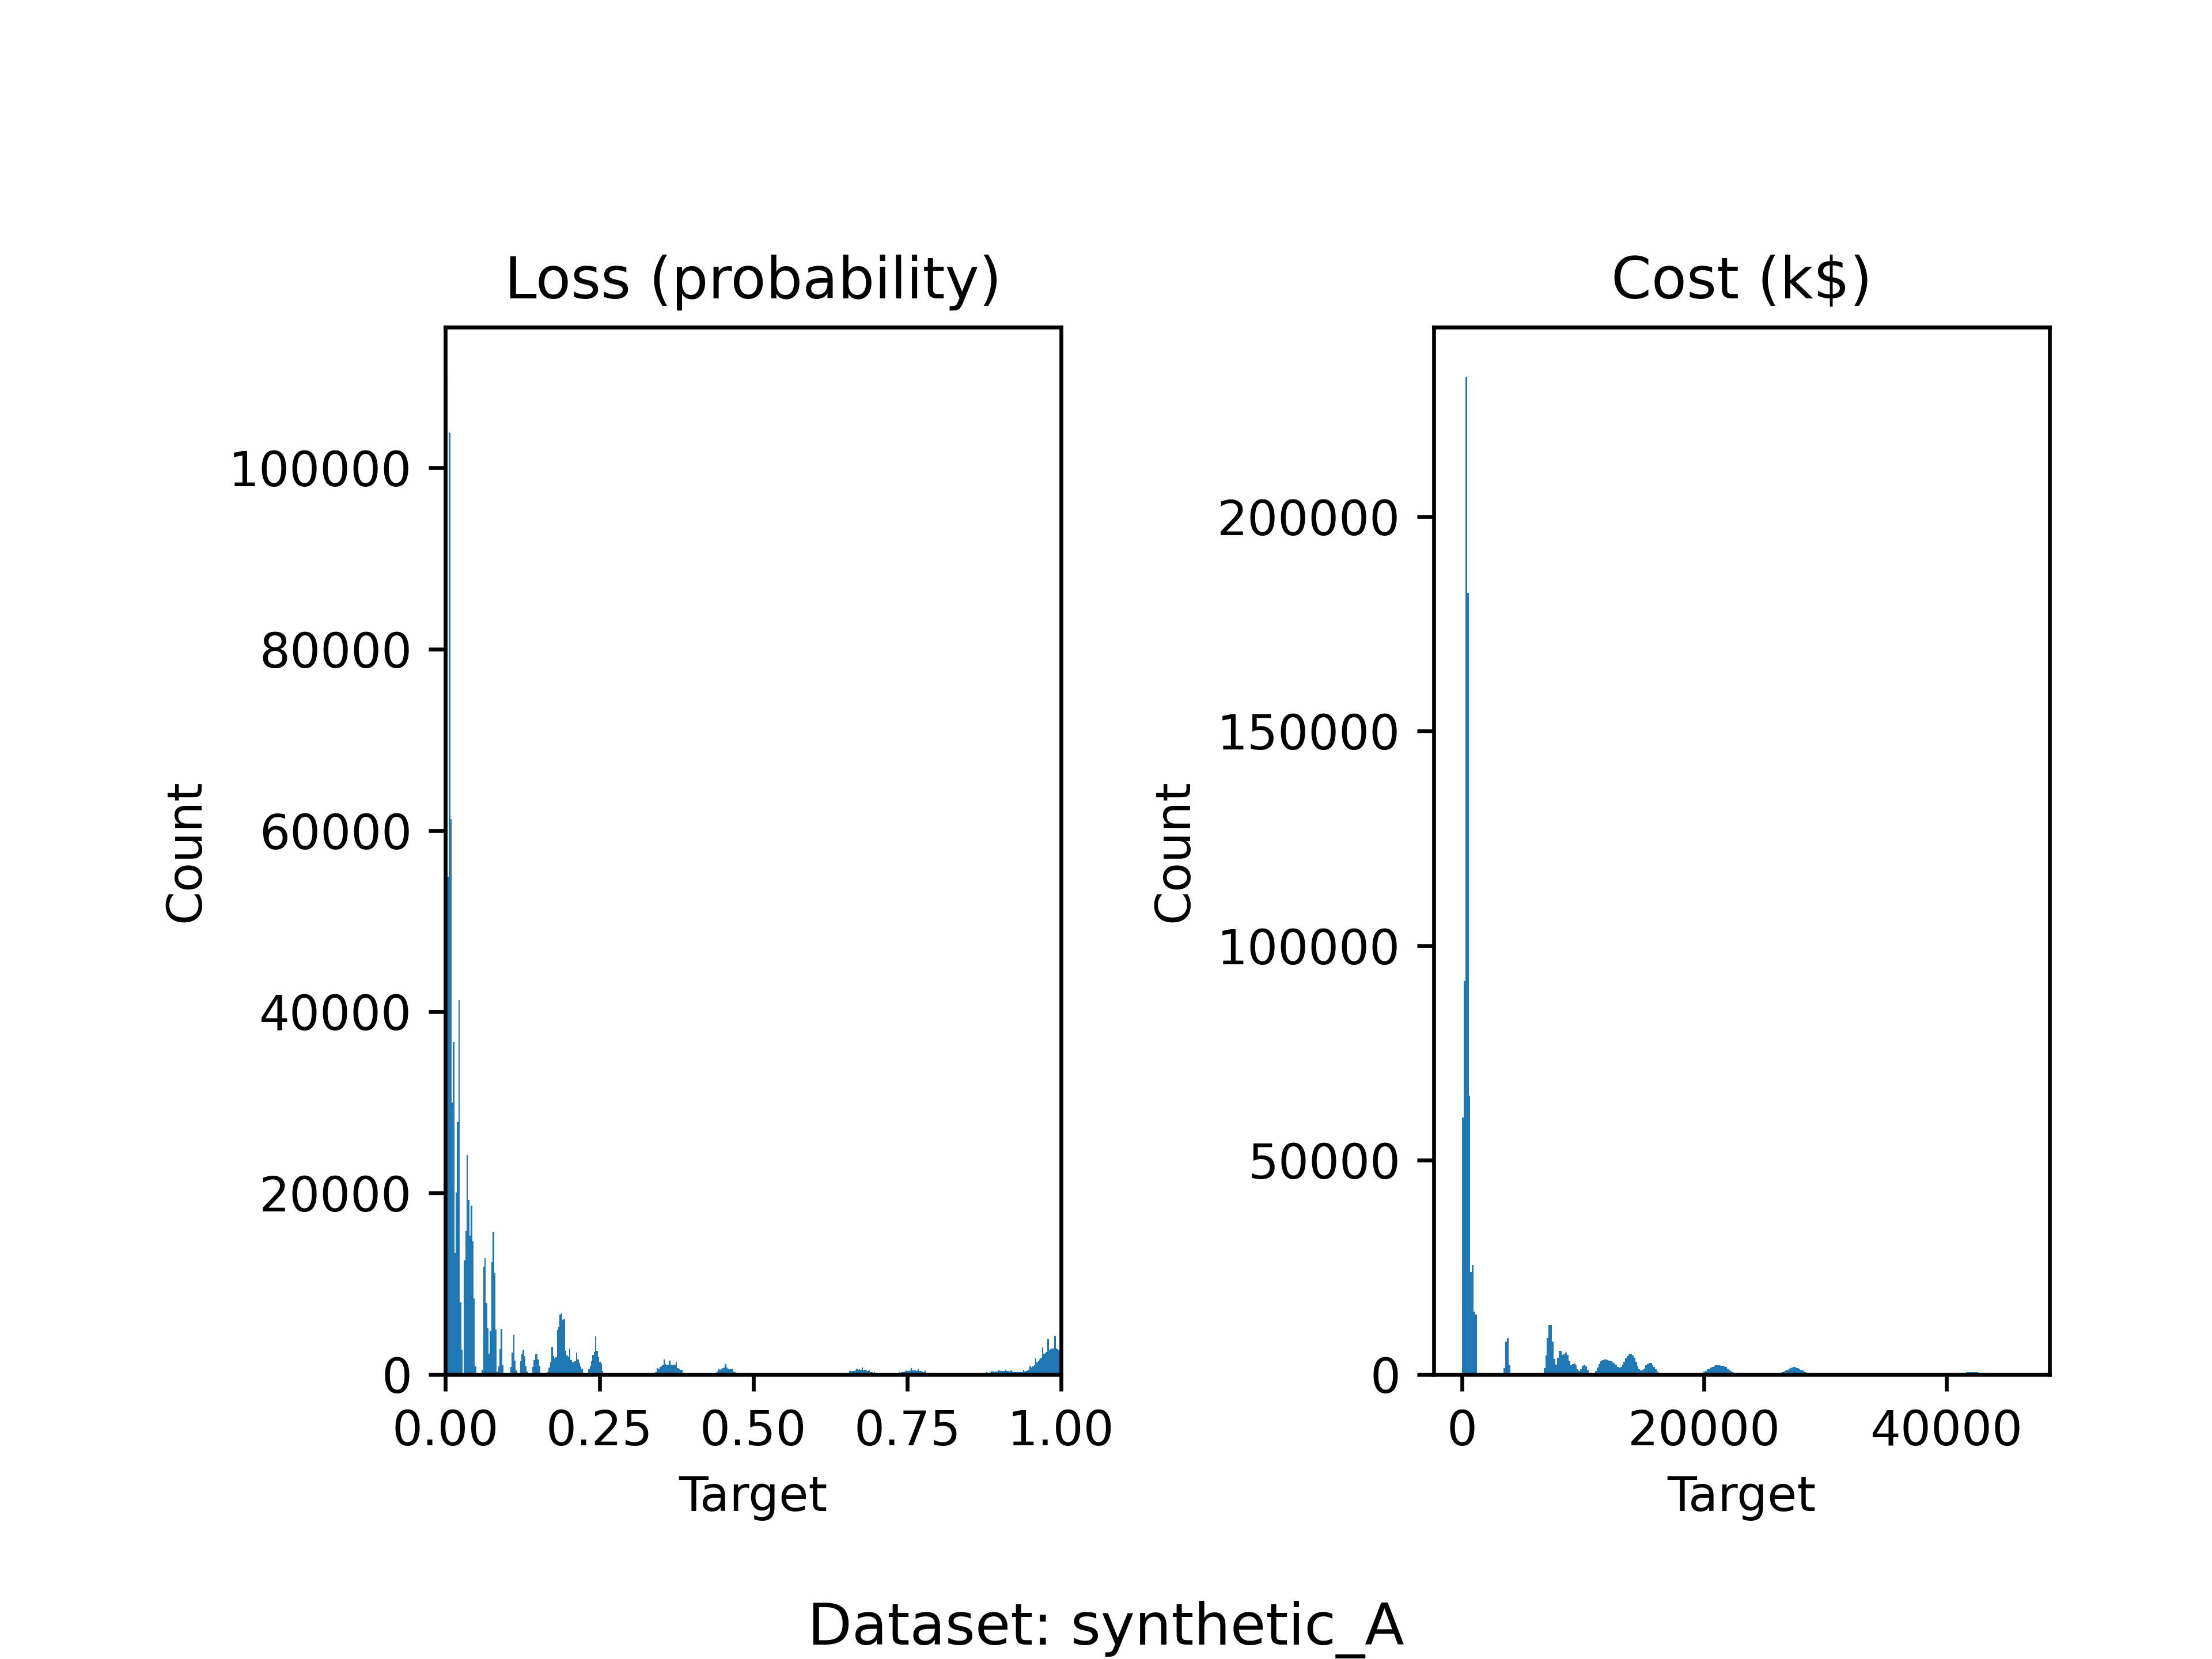
\includegraphics[width=.5\linewidth]{images/synthetic/synthetic_A_histogram.png}\hfill
  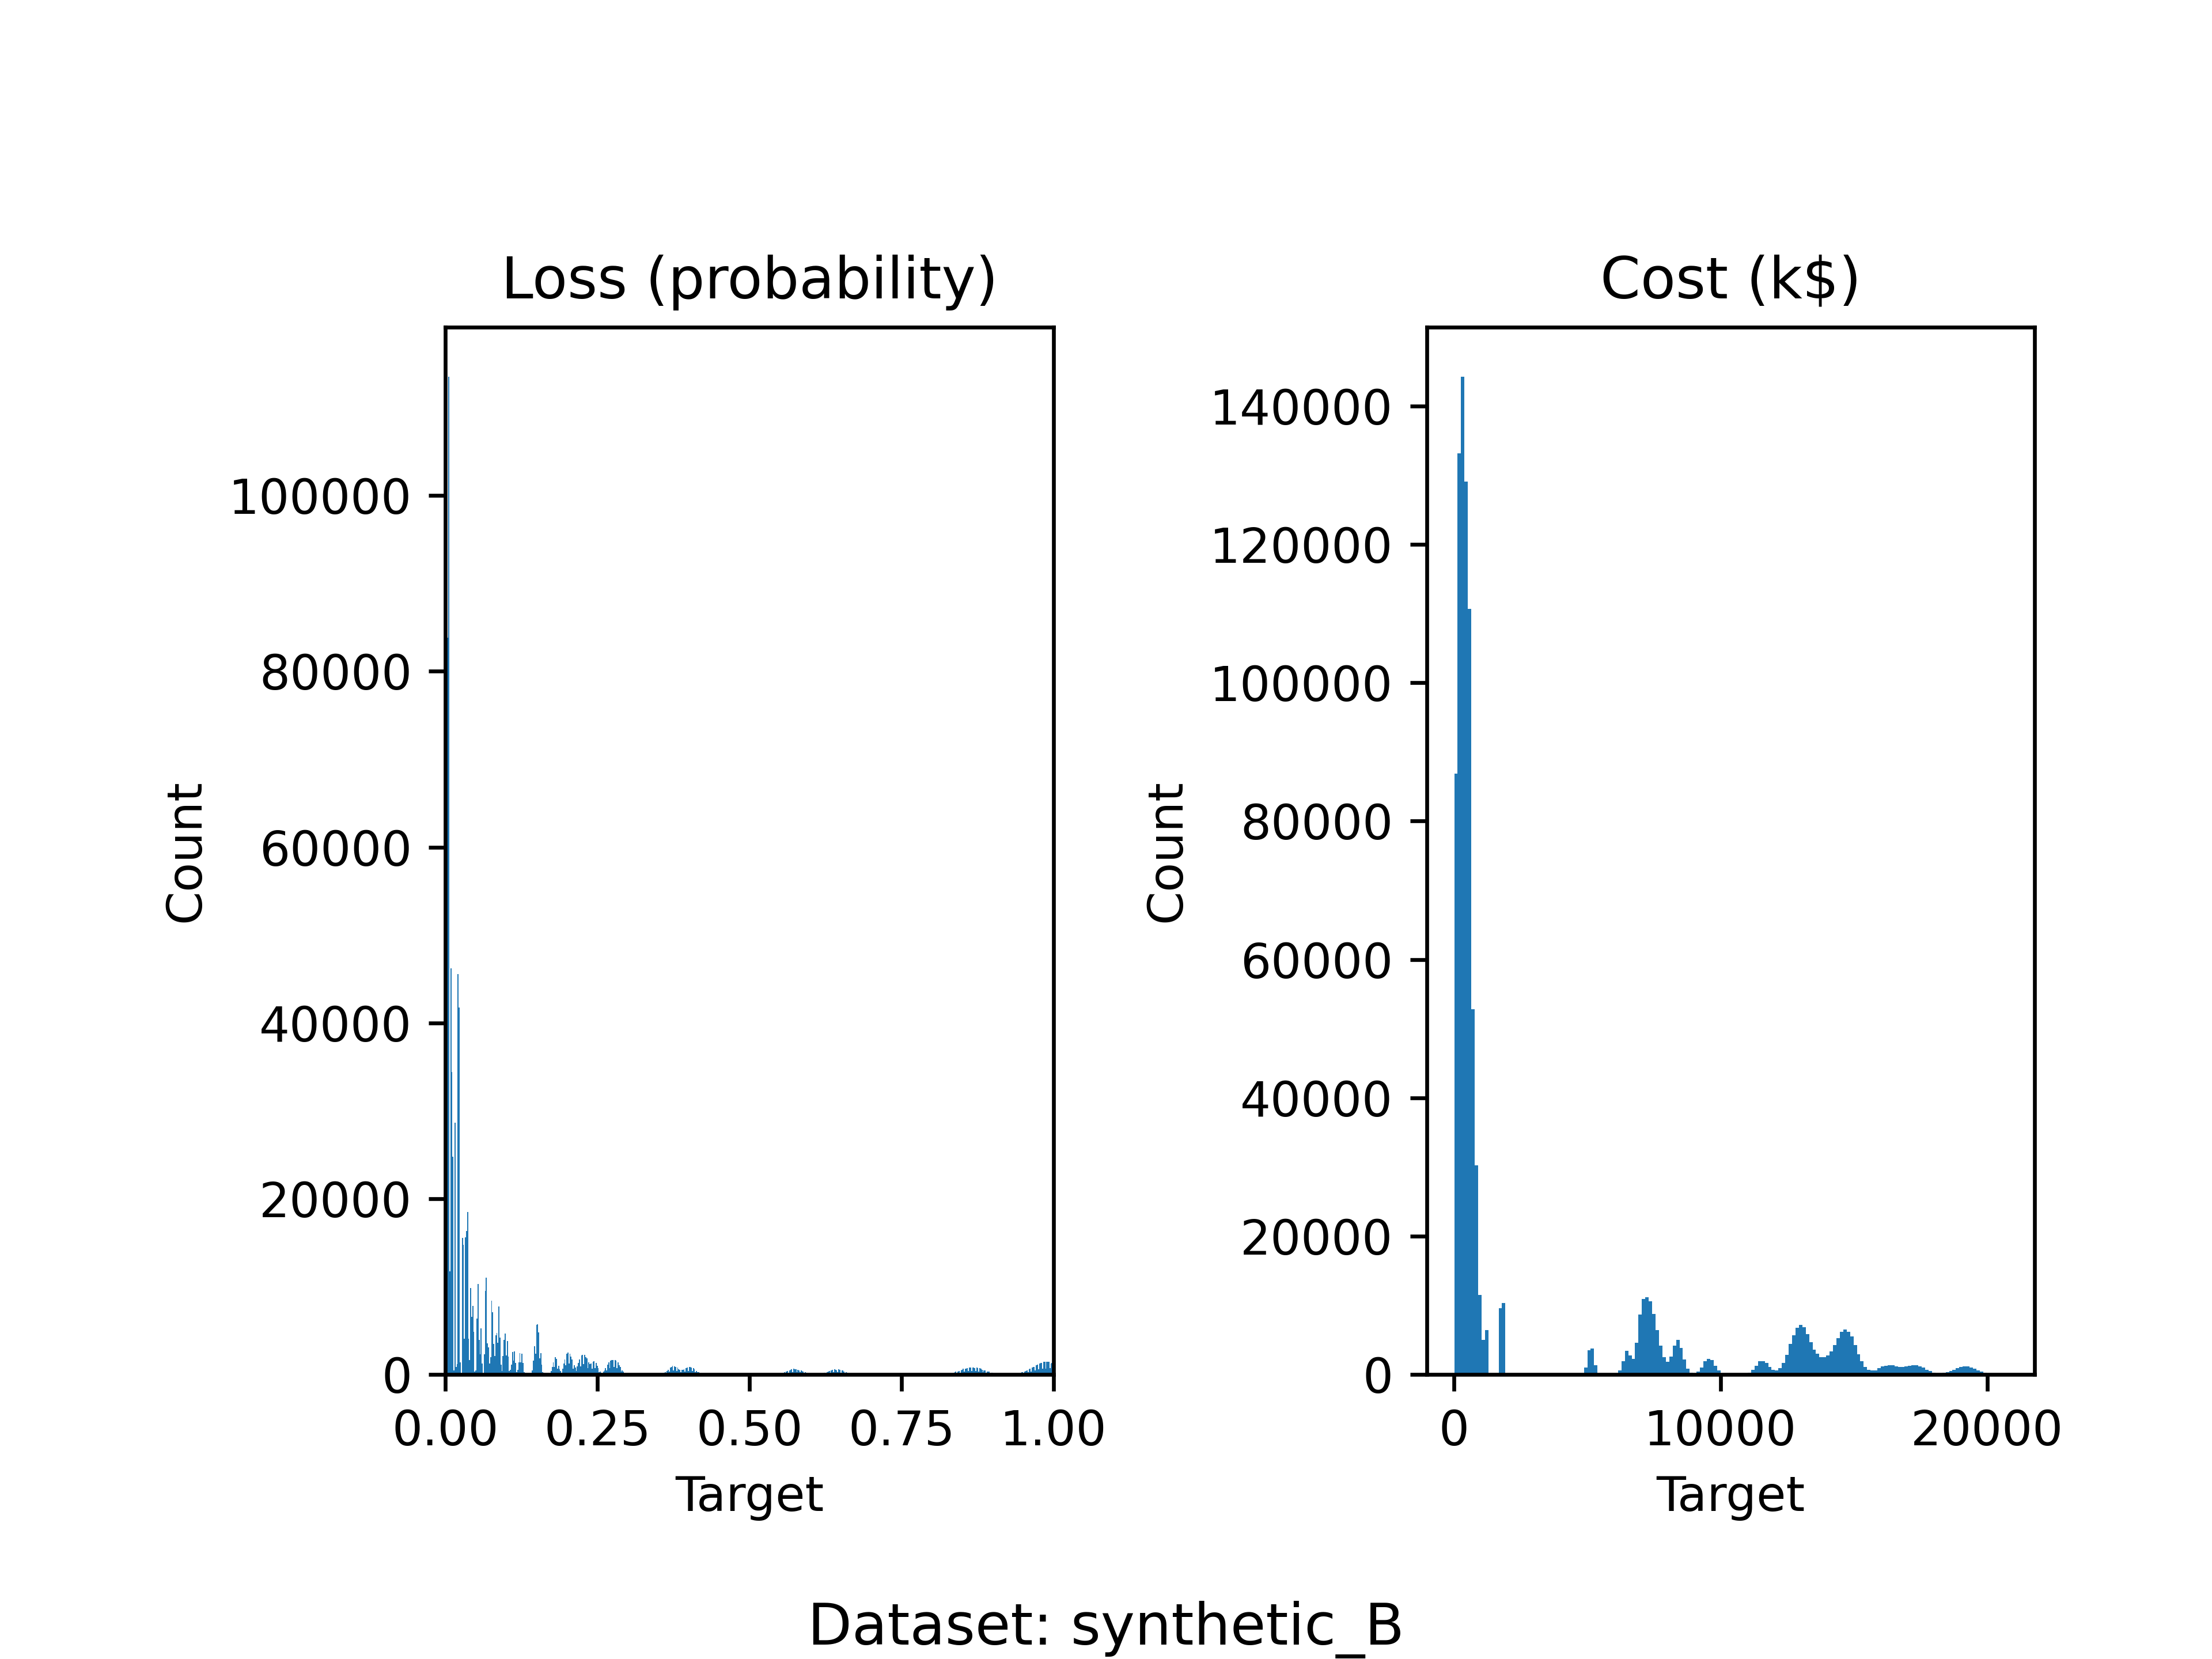
\includegraphics[width=.5\linewidth]{images/synthetic/synthetic_B_histogram.png}
  \caption{Synthetic datasets A and B}
  \end{subfigure}\par\medskip
  \begin{subfigure}{\linewidth}
  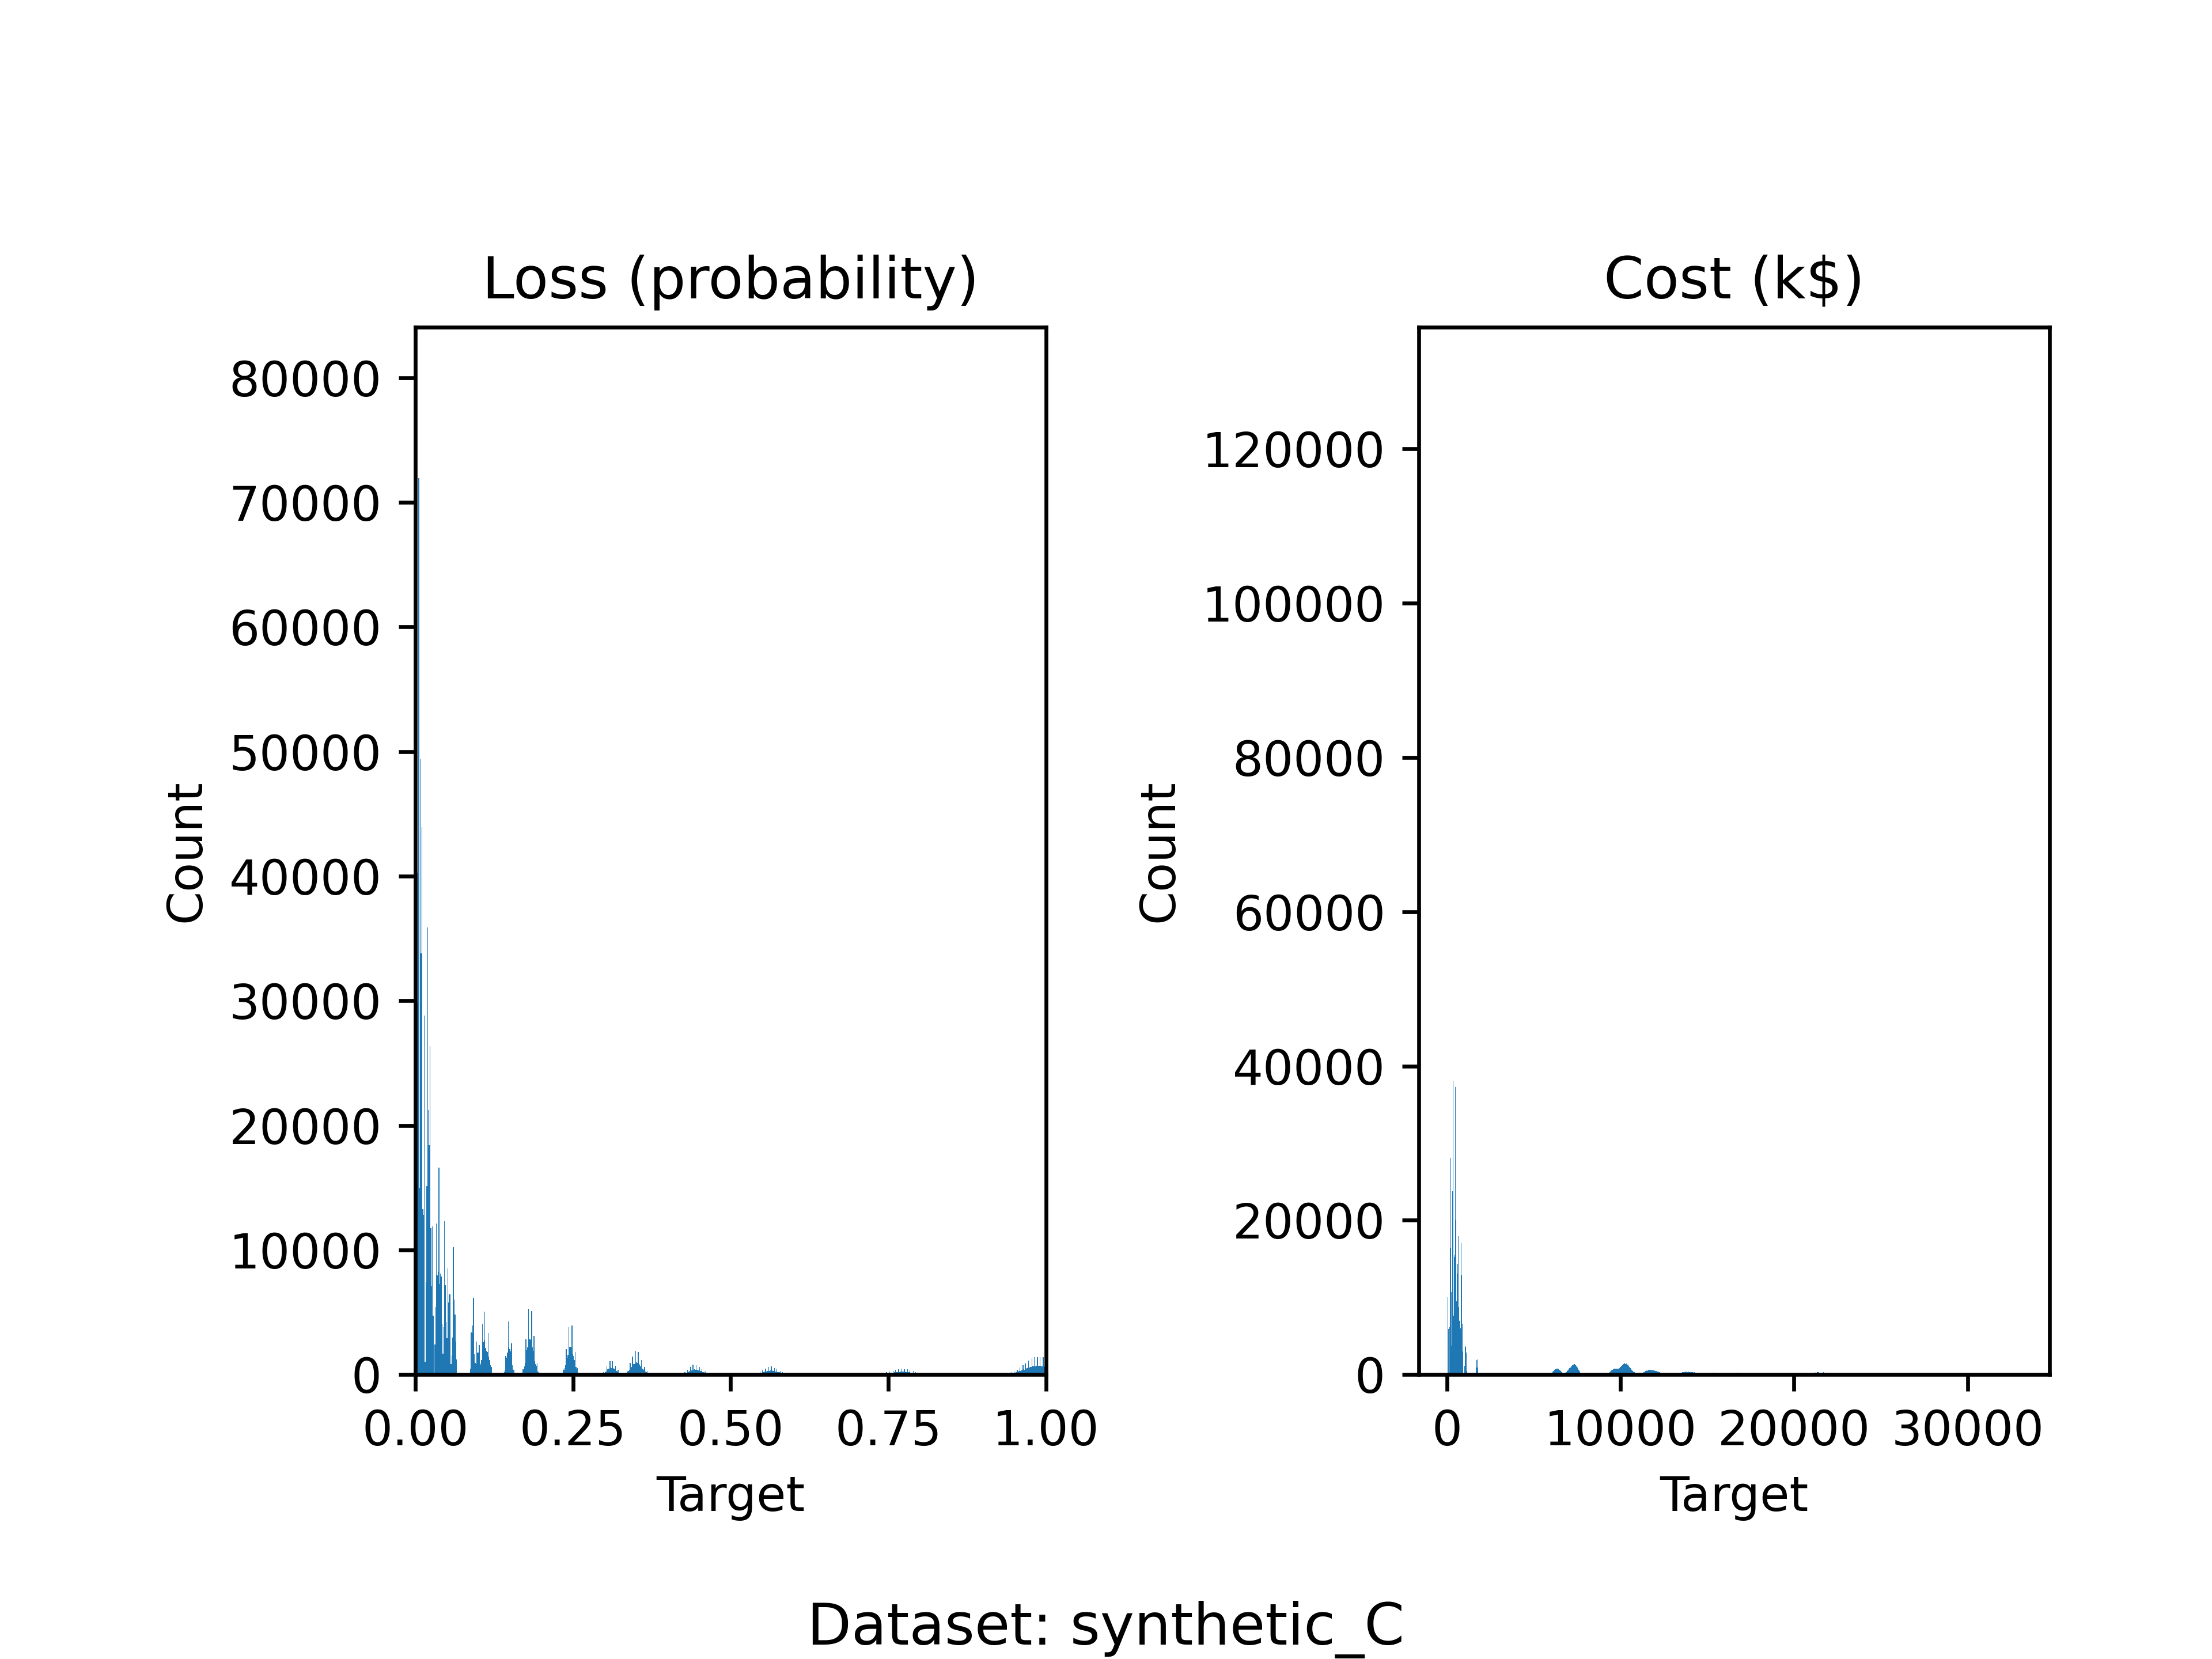
\includegraphics[width=.5\linewidth]{images/synthetic/synthetic_C_histogram.png}\hfill
  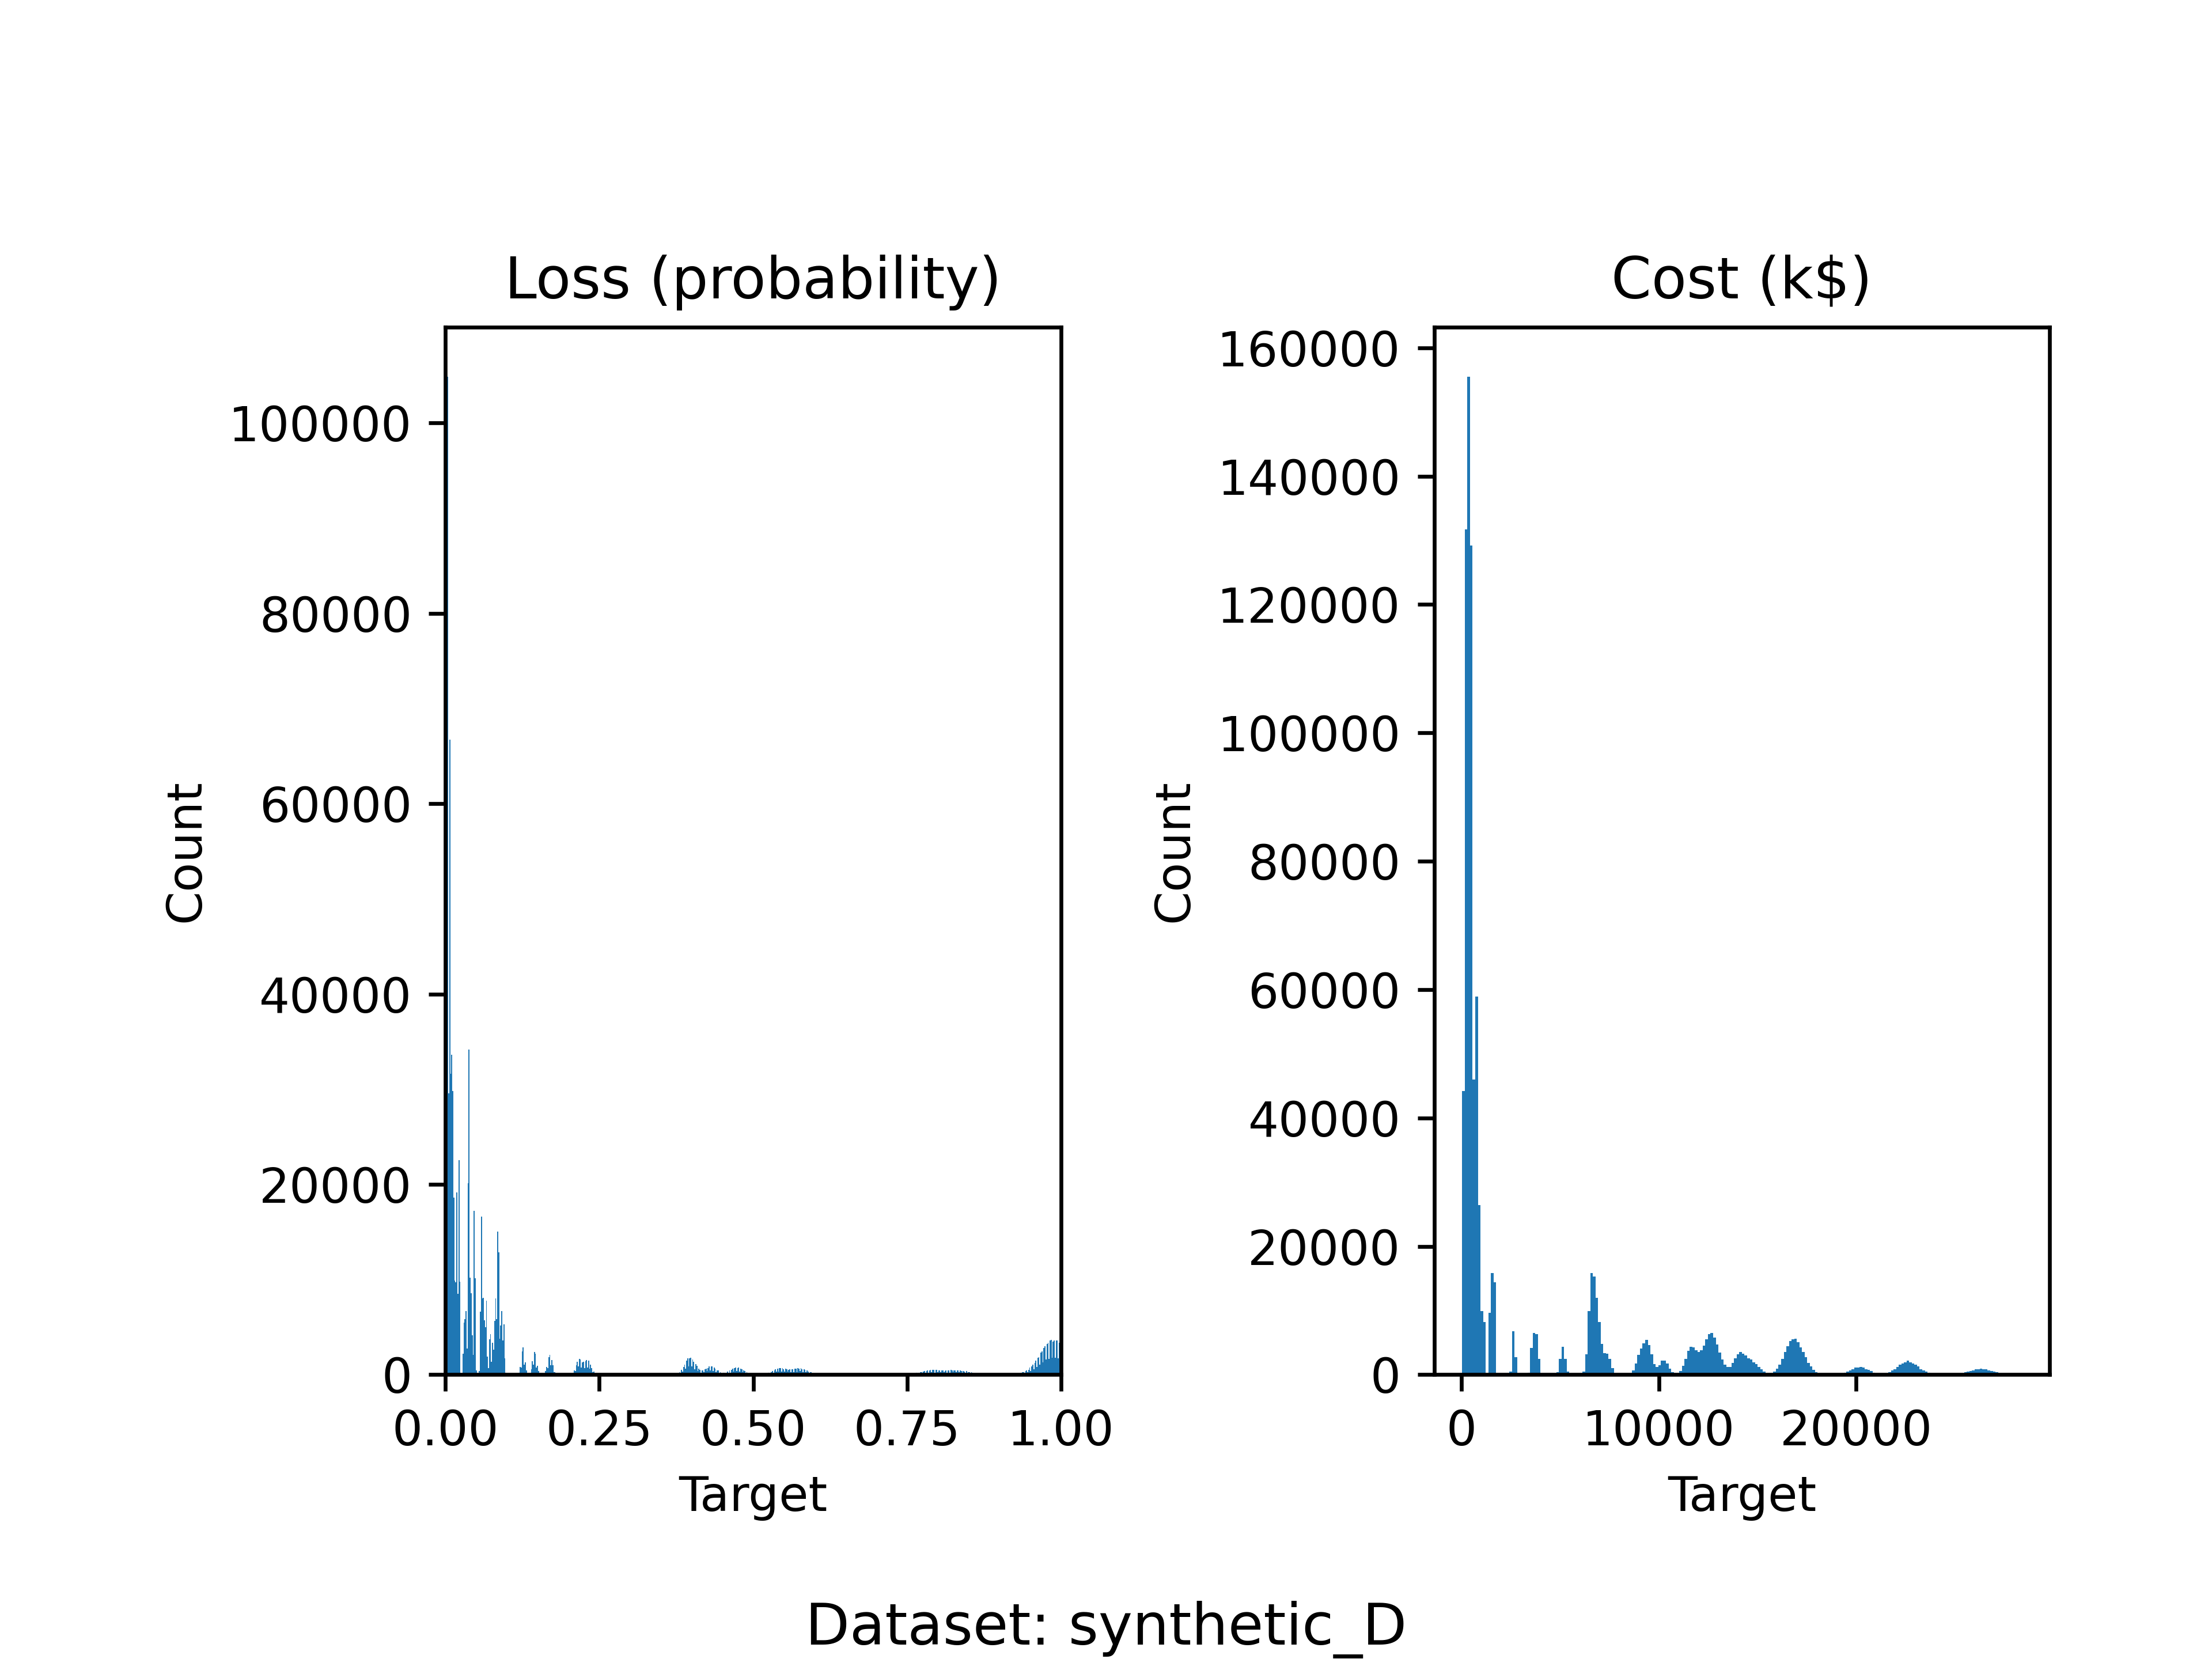
\includegraphics[width=.5\linewidth]{images/synthetic/synthetic_D_histogram.png}
  \caption{Synthetic datasets C and D}
  \end{subfigure}
  \caption{\label{fig:distribution-hard}Target distribution for the synthetic datasets.}
\end{figure}

\begin{figure}[h!]
  \begin{subfigure}{\linewidth}
  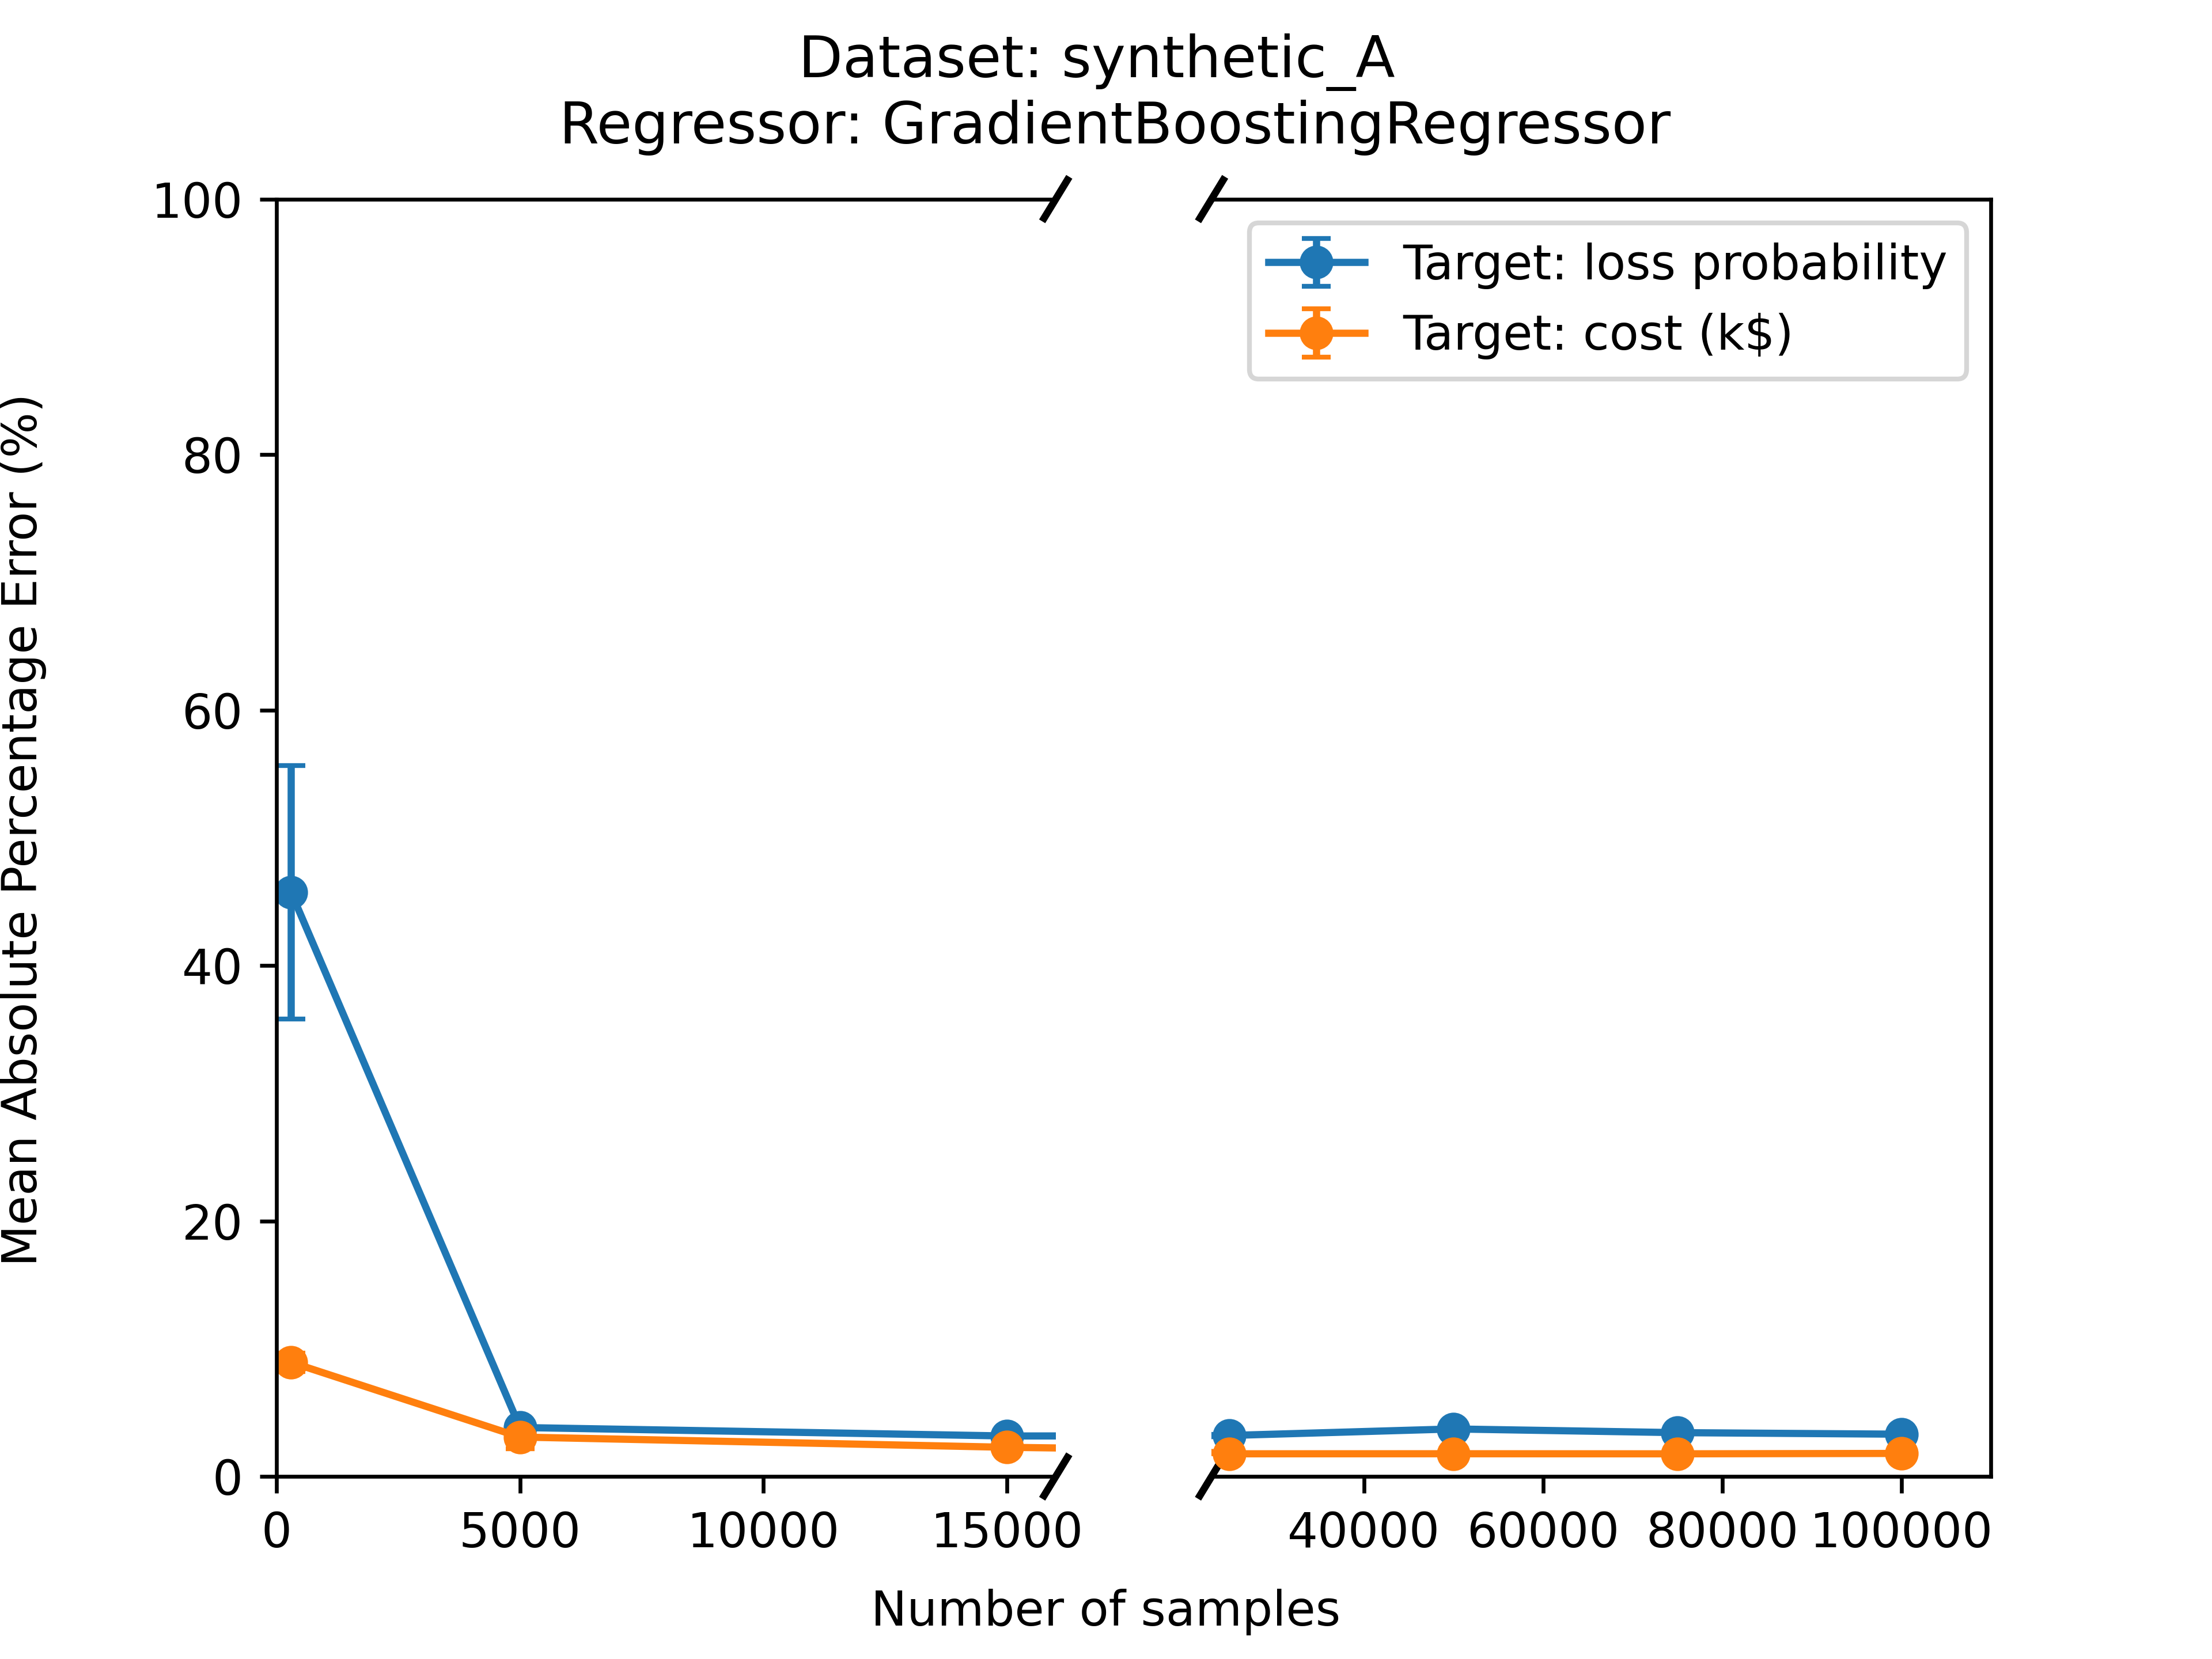
\includegraphics[width=.5\linewidth]{images/synthetic/synthetic_A_complexity.png}\hfill
  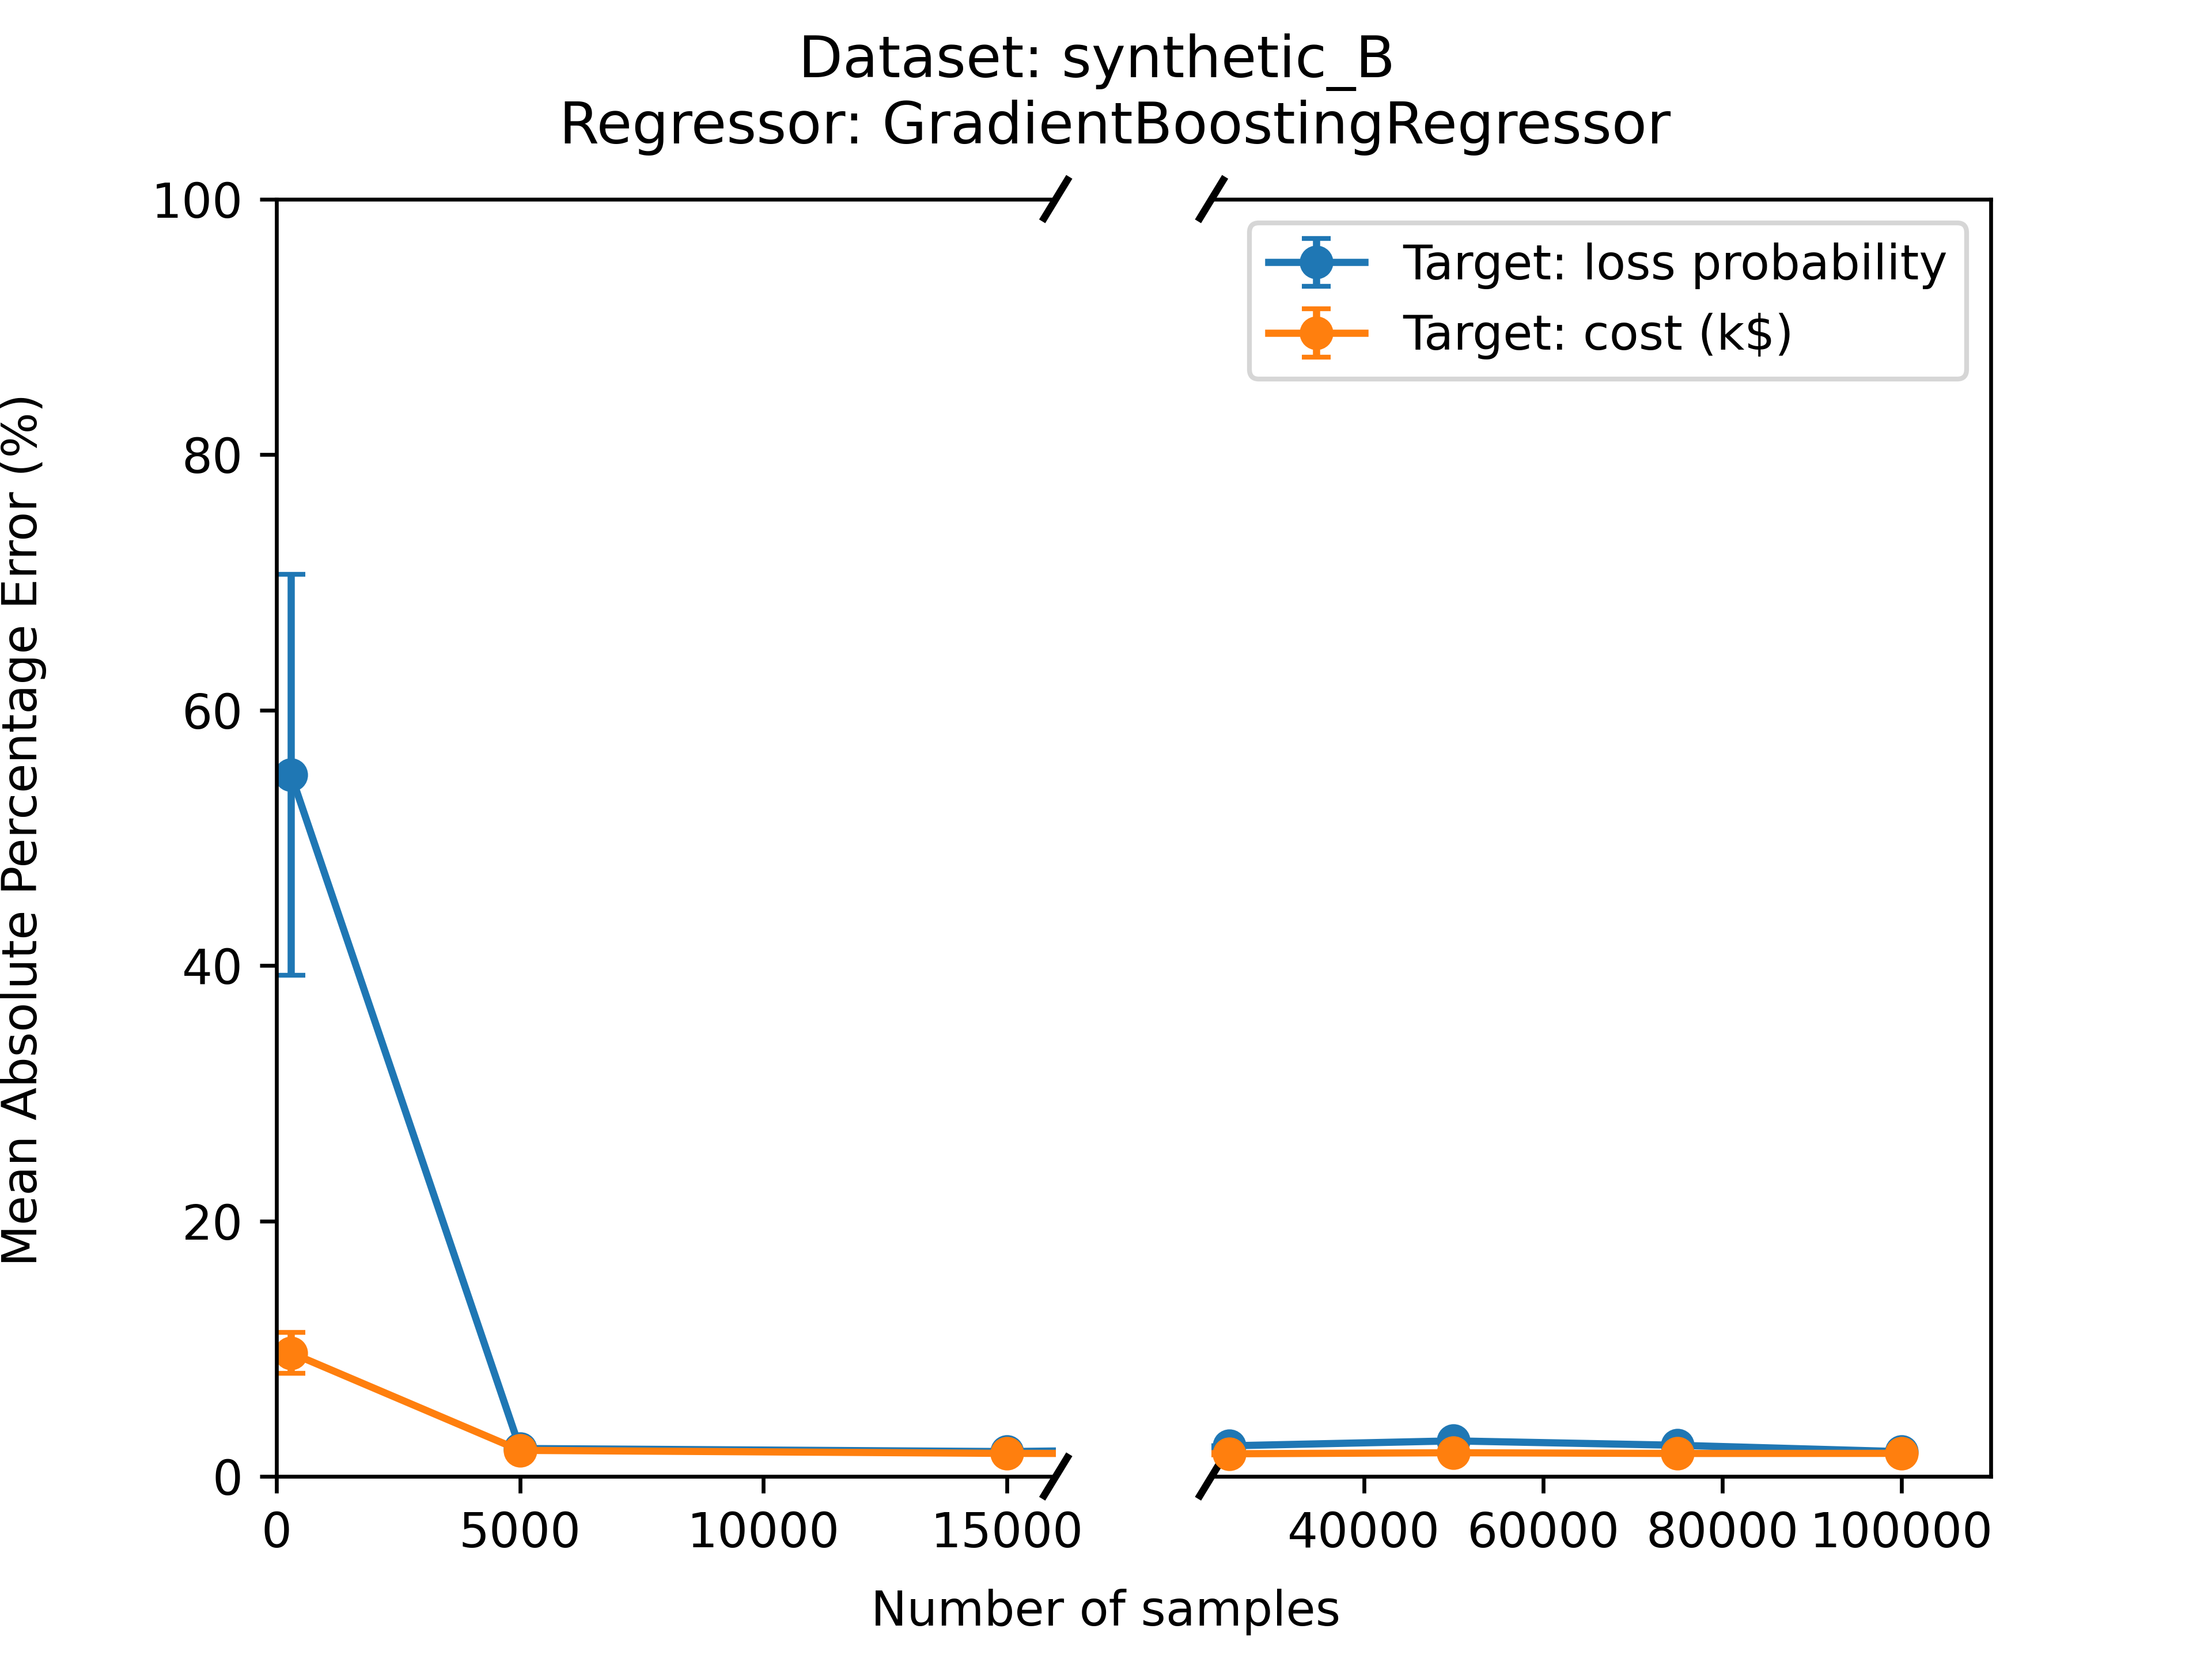
\includegraphics[width=.5\linewidth]{images/synthetic/synthetic_B_complexity.png}
  \caption{Synthetic datasets A and B}
  \end{subfigure}\par\medskip
  \begin{subfigure}{\linewidth}
  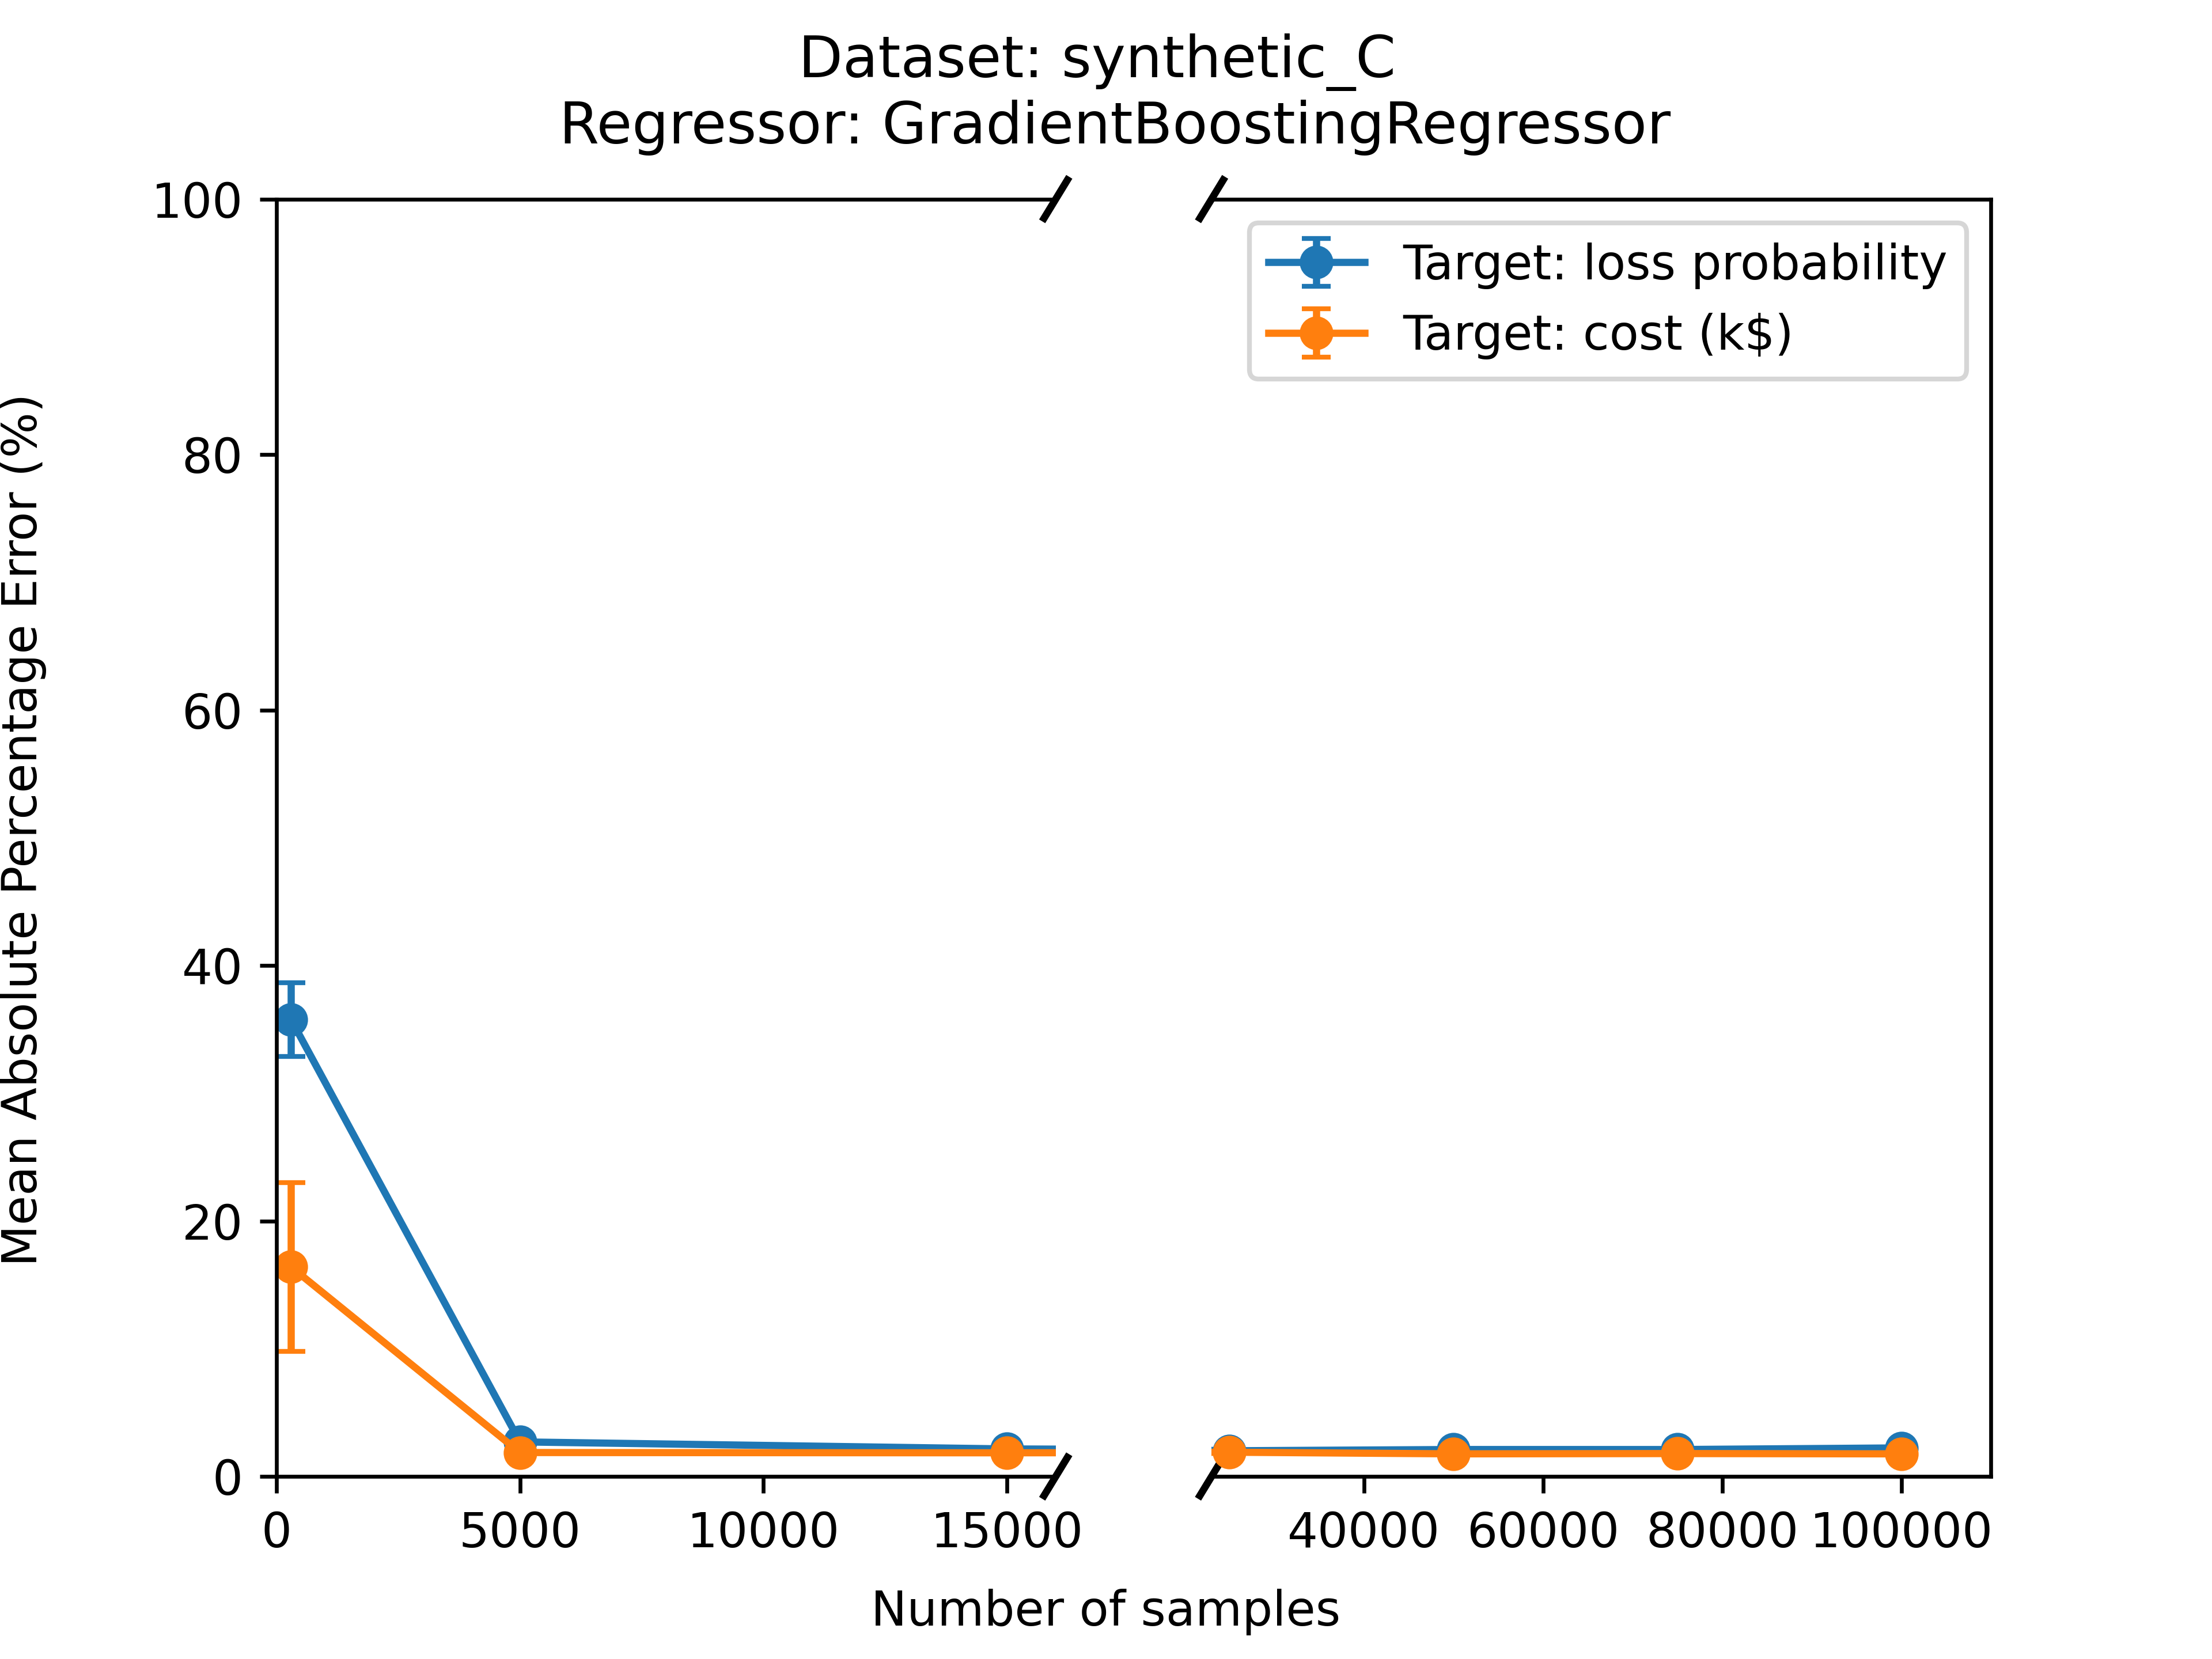
\includegraphics[width=.5\linewidth]{images/synthetic/synthetic_C_complexity.png}\hfill
  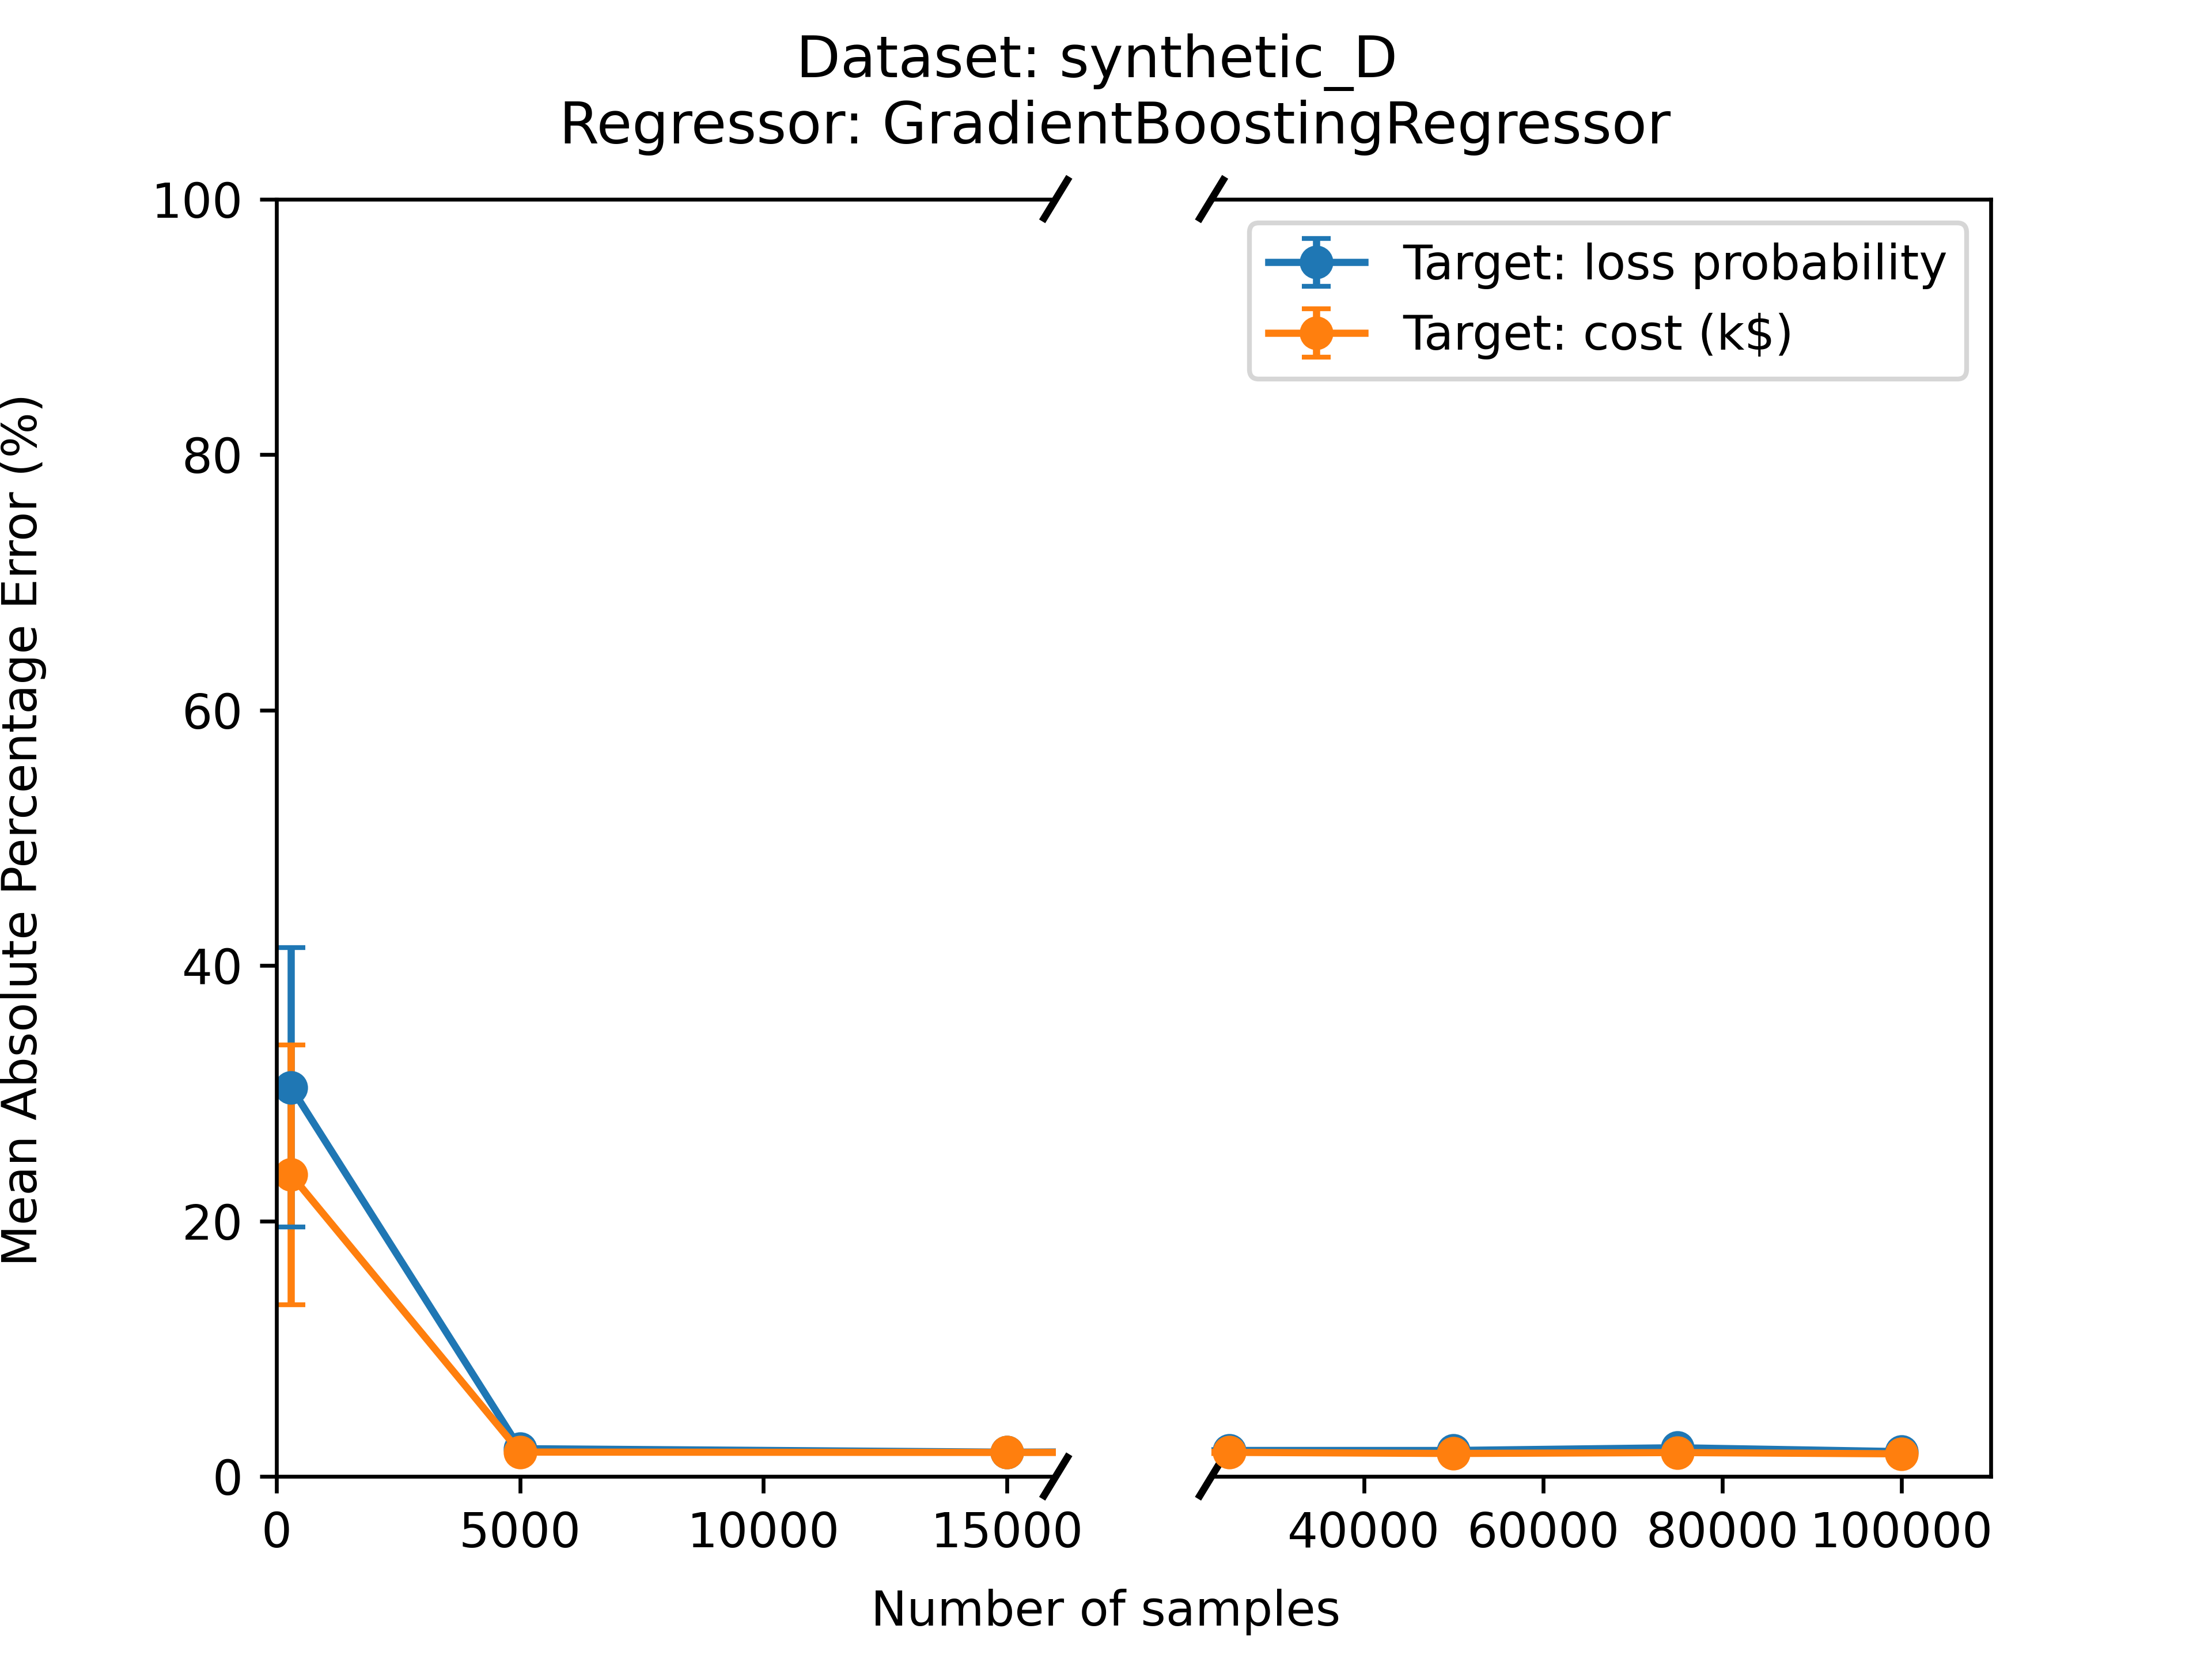
\includegraphics[width=.5\linewidth]{images/synthetic/synthetic_D_complexity.png}
  \caption{Synthetic datasets C and D}
  \end{subfigure}
  \caption{\label{fig:synthetic_data_complexity}Problem difficulty for the synthetic datasets.}
\end{figure}

\begin{center}\begin{table}[h!]
	\center
	\noindent\makebox[0pt]{}{
		\begin{tabular}{|c|c|} 
 		\hline
 		Feature & Meaning \\ [0.5ex] \hline\hline
 		$company\_size$ & One of $[small, \; large]$. Refers to the size of the company. \\ \hline
 		$company\_sector$ & \makecell{The sector the company operates in. Refer to Table ~\ref{table:probs-data} \\ for the list of sectors.} \\ \hline
 		$company\_allows\_BYOD$ & \makecell{The company has a \textit{bring your own device} policy, which \\ allows employees to use their personal devices as their \\ work device. } \\ \hline
 		$company\_does\_pentest$ & \makecell{The company runs penetration tests against their \\ infrastructure, at least once a year.} \\ \hline
 		$company\_uses\_RBAC$ & \makecell{The company has a \textit{role based access control} policy in \\ place.} \\ \hline
 		$company\_does\_red\_teaming$ & The company performs red teaming exercises. \\ \hline
 		$company\_has\_2FA$ & The company uses 2-factor authentication. \\ \hline
 		$company\_has\_password\_policy$ & \makecell{The company has a password policy in place. Such \\ policy defines e.g. the minimum length of \\ employee passwords.} \\ \hline
 		\makecell{$company\_trains\_employees\_$\\$against\_social\_engineering$} & \makecell{The company trains its employees against social \\ engineering techniques. This includes training \\ against e.g. phishing.} \\ \hline
 		$company\_has\_antivirus$ & The company has antivirus in place. \\ \hline
 		$company\_has\_patching\_process$ & \makecell{The company keeps its systems up to date by \\ applying the latest software / security patches \\ on a regular basis.} \\ \hline
 		$company\_has\_ingress\_firewall$ & The company has ingress fire-walling rules. \\ \hline
 		$company\_has\_egress\_firewall$ & The company has egress fire-walling rules. \\ \hline
 		$company\_uses\_3rd\_party$ & \makecell{The company relies on a 3rd party provider for some \\ of its services. This can be e.g. cloud-based solutions.} \\ \hline
 		$company\_has\_ciso$ & The company has a dedicated CISO. \\ \hline
 		\makecell{$company\_has\_threat\_$\\$intelligence\_team$} & The company has a dedicated threat intelligence team. \\ \hline
 		$company\_monitors\_IOCs$ & \makecell{The company is subscribed to an indicator of \\ compromise feed.} \\ \hline
 		$company\_has\_IDS$ & The company has an intrusion detection system. \\ \hline
 		$company\_has\_IPS$ & The company has an intrusion prevention system. \\ \hline
 		$company\_separates\_systems$ & \makecell{The company separates its systems, e.g. they have a \\ DMZ. } \\ \hline
 		$company\_does\_daily\_backup$ & The company performs daily backups of its systems. \\ \hline
 		$company\_has\_recovery\_plan$ & \makecell{In the event of a security incident or other disaster, \\ the company has a process for recovery in place. \\ This can include people to contact, processes to start, etc.} \\ \hline
 		\makecell{$company\_has\_incident\_$\\$response\_team$} & The company has a dedicated IR team. \\ \hline
	\end{tabular}
	\caption{\label{table:features_meaning} List of features and their meaning for the synthetic datasets.}}
\end{table}\end{center}

\begin{center}\begin{table}[h!]
	\center
	\noindent\makebox[0pt]{}{
		\begin{tabular}{|c|c|c|} 
 		\hline
 		Feature ($F$) & $P(F)$ & $P(F|loss)$ \\ [0.5ex] \hline\hline
 		$company\_size$ & \makecell{small: 0.68 \\ large: 0.32} & \\ \hline
 		$company\_sector$ & See Table ~\ref{table:probs} & \\ \hline
 		$company\_allows\_BYOD$ & 0.44 & 0.14 \\ \hline
 		$company\_does\_pentest$ & 0.36 & 0.23 \\ \hline
 		$company\_uses\_RBAC$ & 0.85 & 0.67 \\ \hline
 		$company\_does\_red\_teaming$ & 0.33 & \\ \hline
 		$company\_has\_2FA$ & 0.78 & \\ \hline
 		$company\_has\_password\_policy$ & 0.88 & \\ \hline
 		\makecell{$company\_trains\_employees\_$\\$against\_social\_engineering$} & 0.70 & \\ \hline
 		$company\_has\_antivirus$ & 0.95 & 0.81 \\ \hline
 		$company\_has\_patching\_process$ & 0.60 & 0.828 \\ \hline
 		$company\_has\_ingress\_firewall$ & 0.83 & 0.84 \\ \hline
 		$company\_has\_egress\_firewall$ & 0.61 & 0.76 \\ \hline
 		$company\_uses\_3rd\_party$ & 0.87 & 0.79 \\ \hline
 		$company\_has\_ciso$ & 0.67 & 0.68 \\ \hline
 		\makecell{$company\_has\_threat\_$\\$intelligence\_team$} & 0.38 & \\ \hline
 		$company\_monitors\_IOCs$ & 0.44 & \\ \hline
 		$company\_has\_IDS$ & 0.94 & \\ \hline
 		$company\_has\_IPS$ & 0.81 & \\ \hline
 		$company\_separates\_systems$ & 0.79 & \\ \hline
 		$company\_does\_daily\_backup$ & 0.91 & \\ \hline
 		$company\_has\_recovery\_plan$ & 0.33 & \\ \hline
 		\makecell{$company\_has\_incident\_$\\$response\_team$} & 0.46& \\ \hline
	\end{tabular}
	\caption{\label{table:all_probs} List of probabilities used in the Bayesian Network in Figure ~\ref{fig:bayesian-hard}. Conditional probabilities that rely on multiple features are omitted but are available in the implementation.}}
\end{table}\end{center}

\begin{center}\begin{table}[h!]
	\center
	\noindent\makebox[0pt]{}{
		\begin{tabular}{|c|c|c|c|}
 		\hline
 		 & (Non-DP) Vanilla & (DP) Depth-first & (DP) 2-nodes \\ [0.5ex] \hline\hline
 		Synthetic A (MAPE) & $3.71 \pm 0.37 $ & $\textbf{10.3}5 \pm \textbf{0.76} $  & $10.92 \pm 1.61 $ \\ \hline
 		Synthetic B (MAPE) & $3.05 \pm 0.49$ & $\textbf{9.35} \pm \textbf{1.69}$  & $11.97 \pm 2.11$ \\ \hline
 		Synthetic C (MAPE) & $2.33 \pm 0.23$ & $9.25 \pm 0.56$  & $\textbf{9.24} \pm \textbf{1.13}$ \\ \hline
 		Synthetic D (MAPE) & $3.00 \pm 0.83$ & $\textbf{13.08} \pm \textbf{1.54}$  & $16.06 \pm 4.06$ \\ \hline
	\end{tabular}
	\caption{\label{table:pred_results_synthetic_loss} Prediction error for the \textit{loss} target on the synthetic datasets.}}
\end{table}\end{center}

\begin{figure}[h!]
  \begin{subfigure}{\linewidth}
  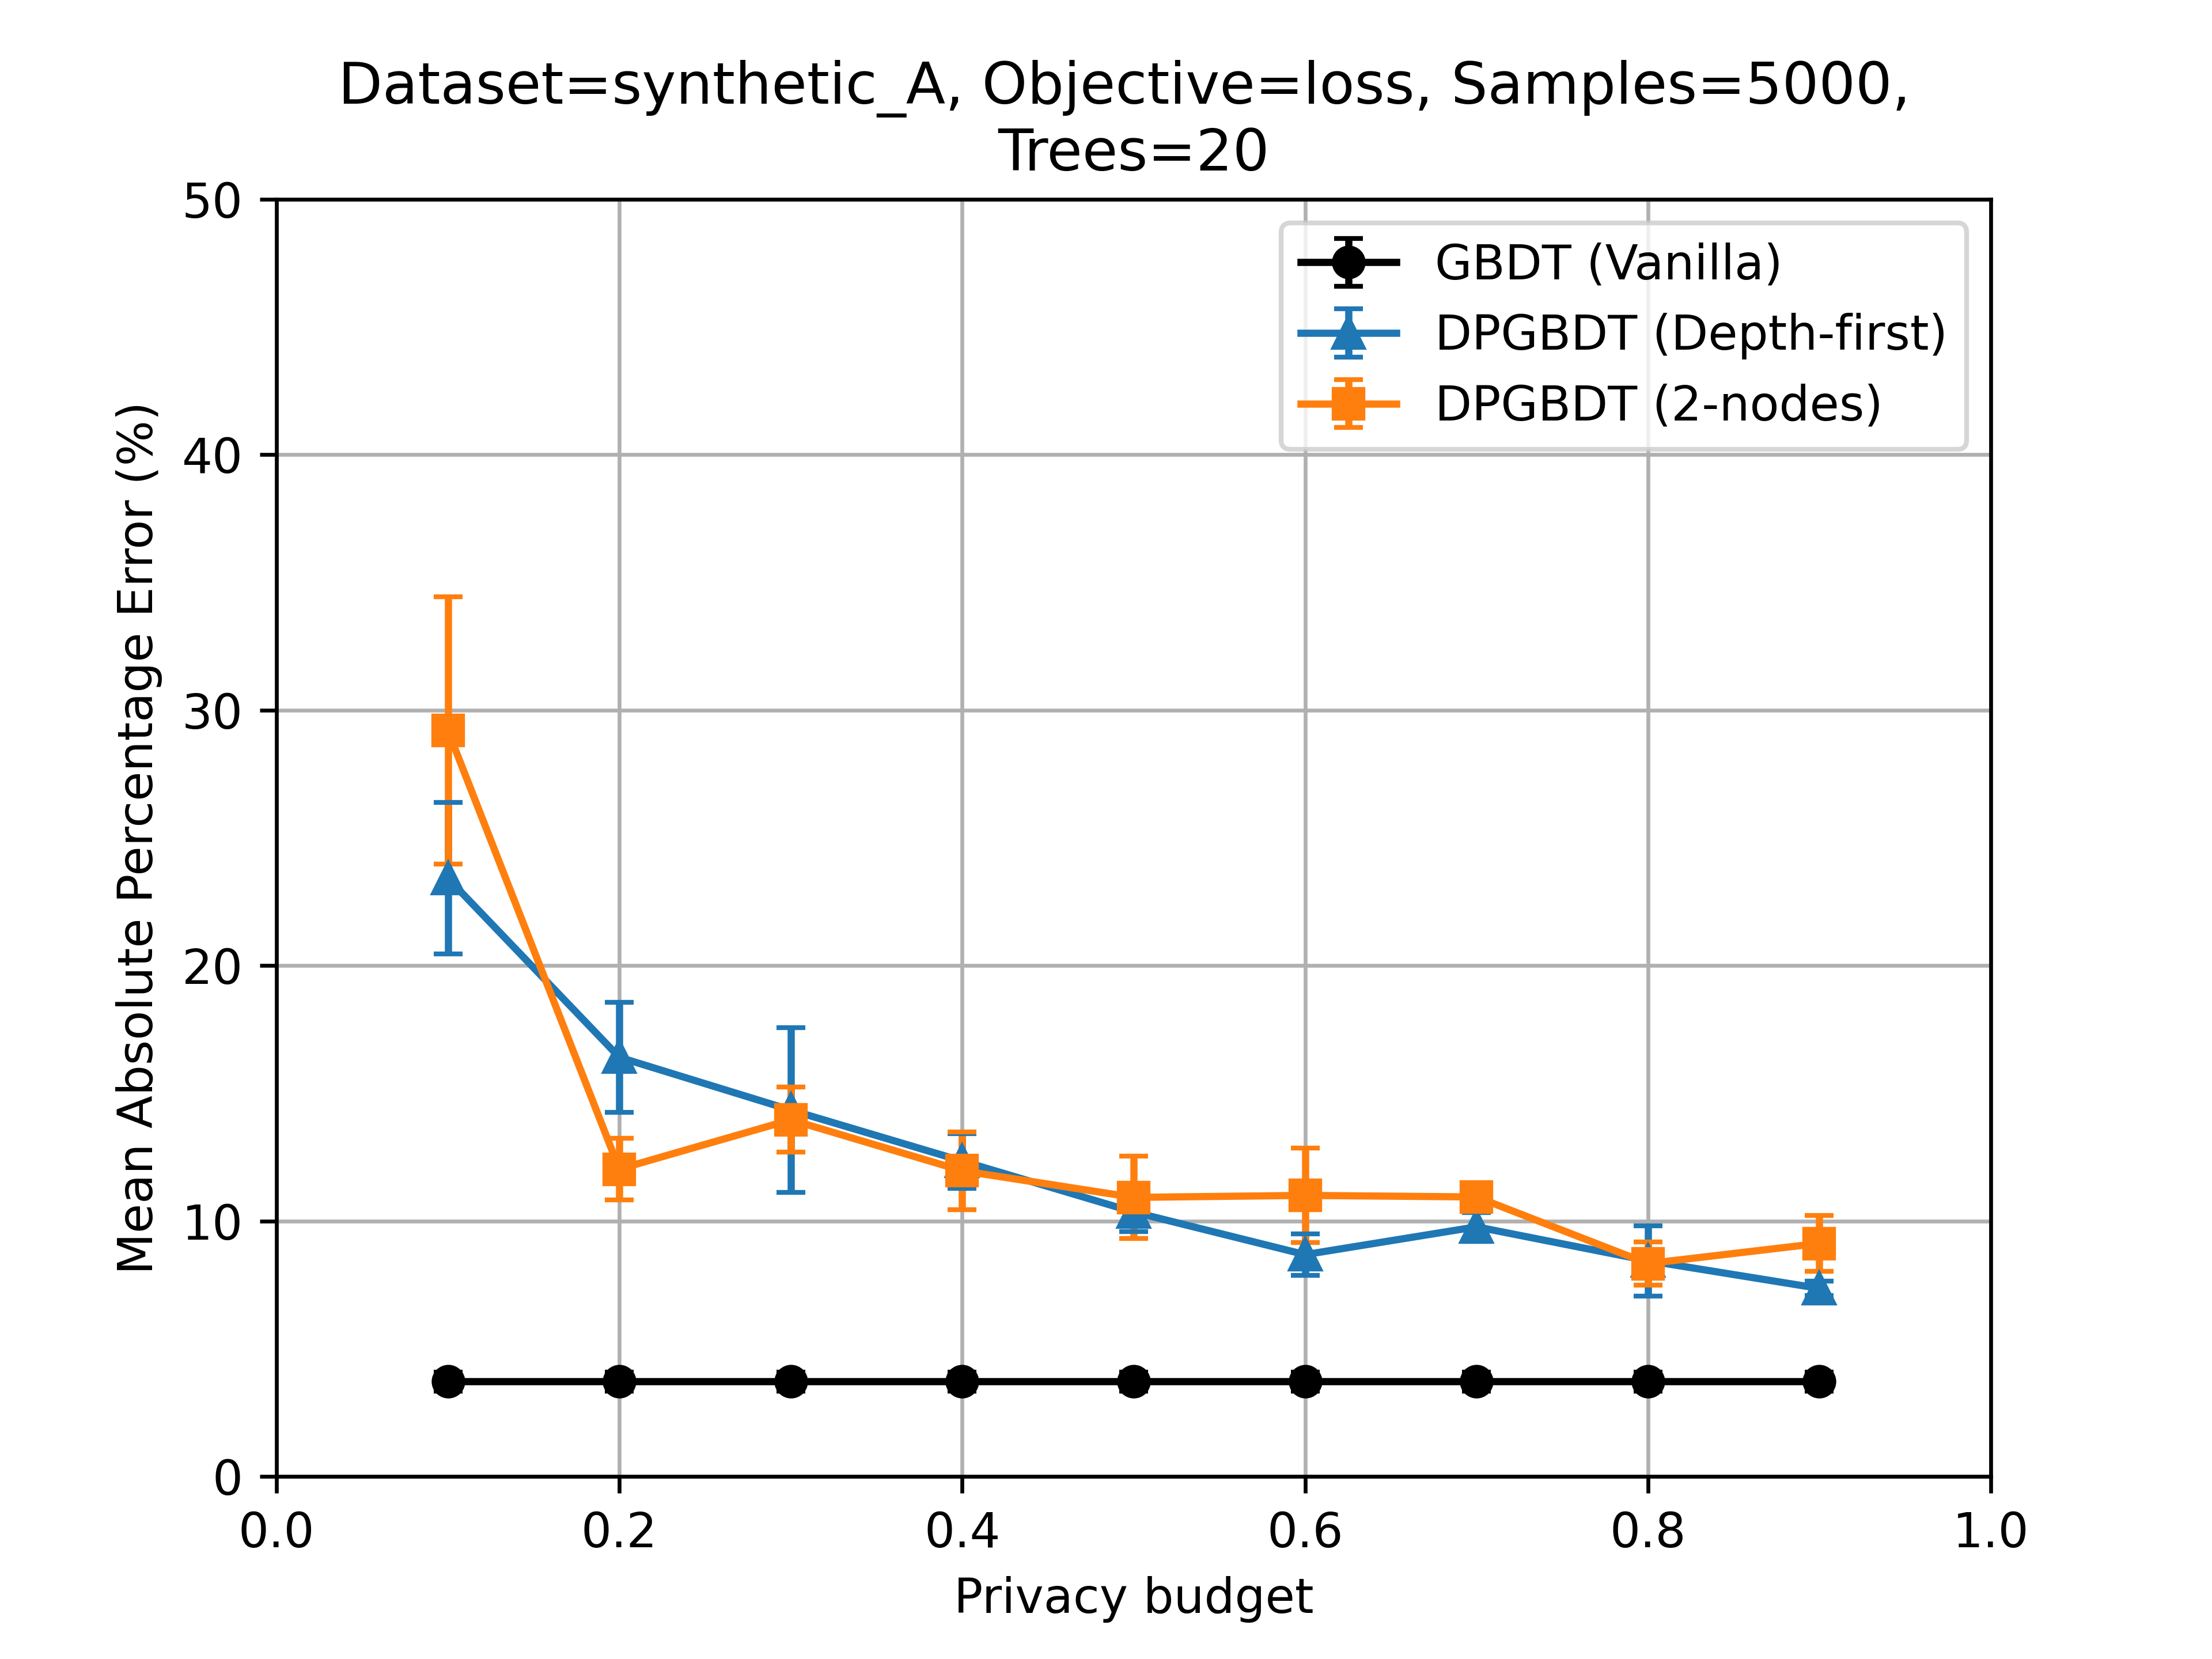
\includegraphics[width=.5\linewidth]{images/evaluation/synthetic_A_loss_5000.png}\hfill
  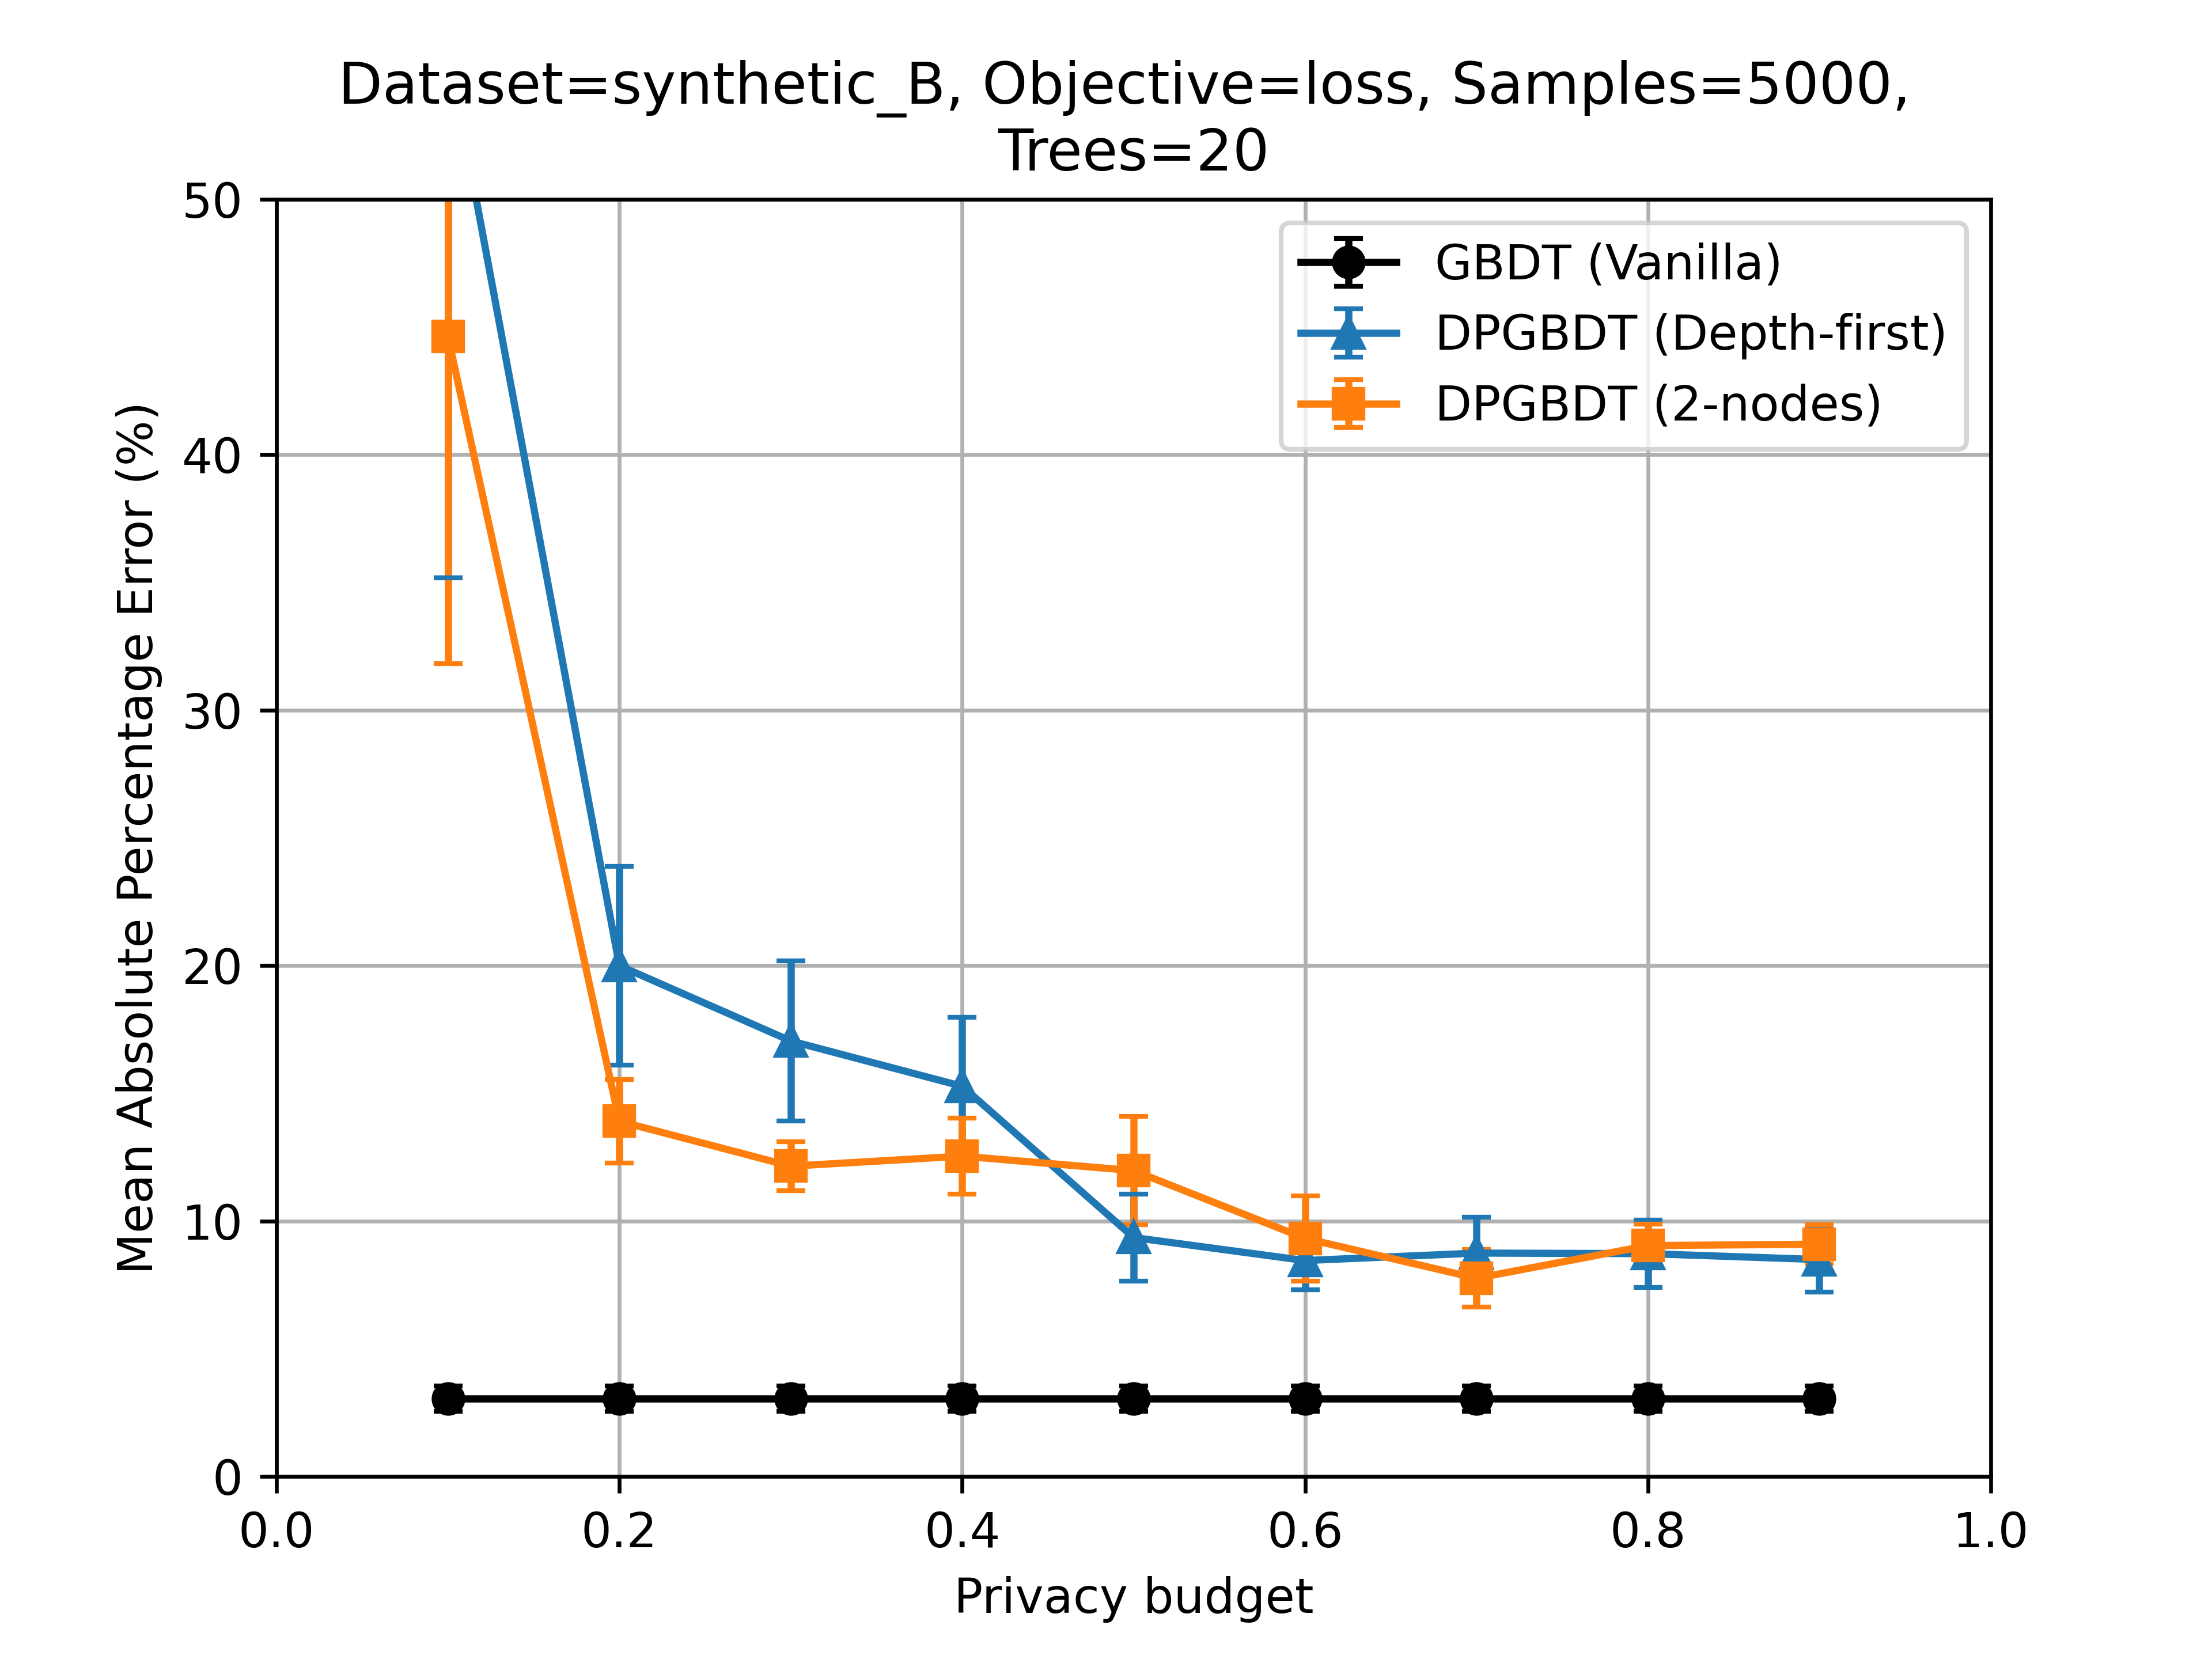
\includegraphics[width=.5\linewidth]{images/evaluation/synthetic_B_loss_5000.png}
  \caption{Synthetic datasets A and B}
  \end{subfigure}\par\medskip
  \begin{subfigure}{\linewidth}
  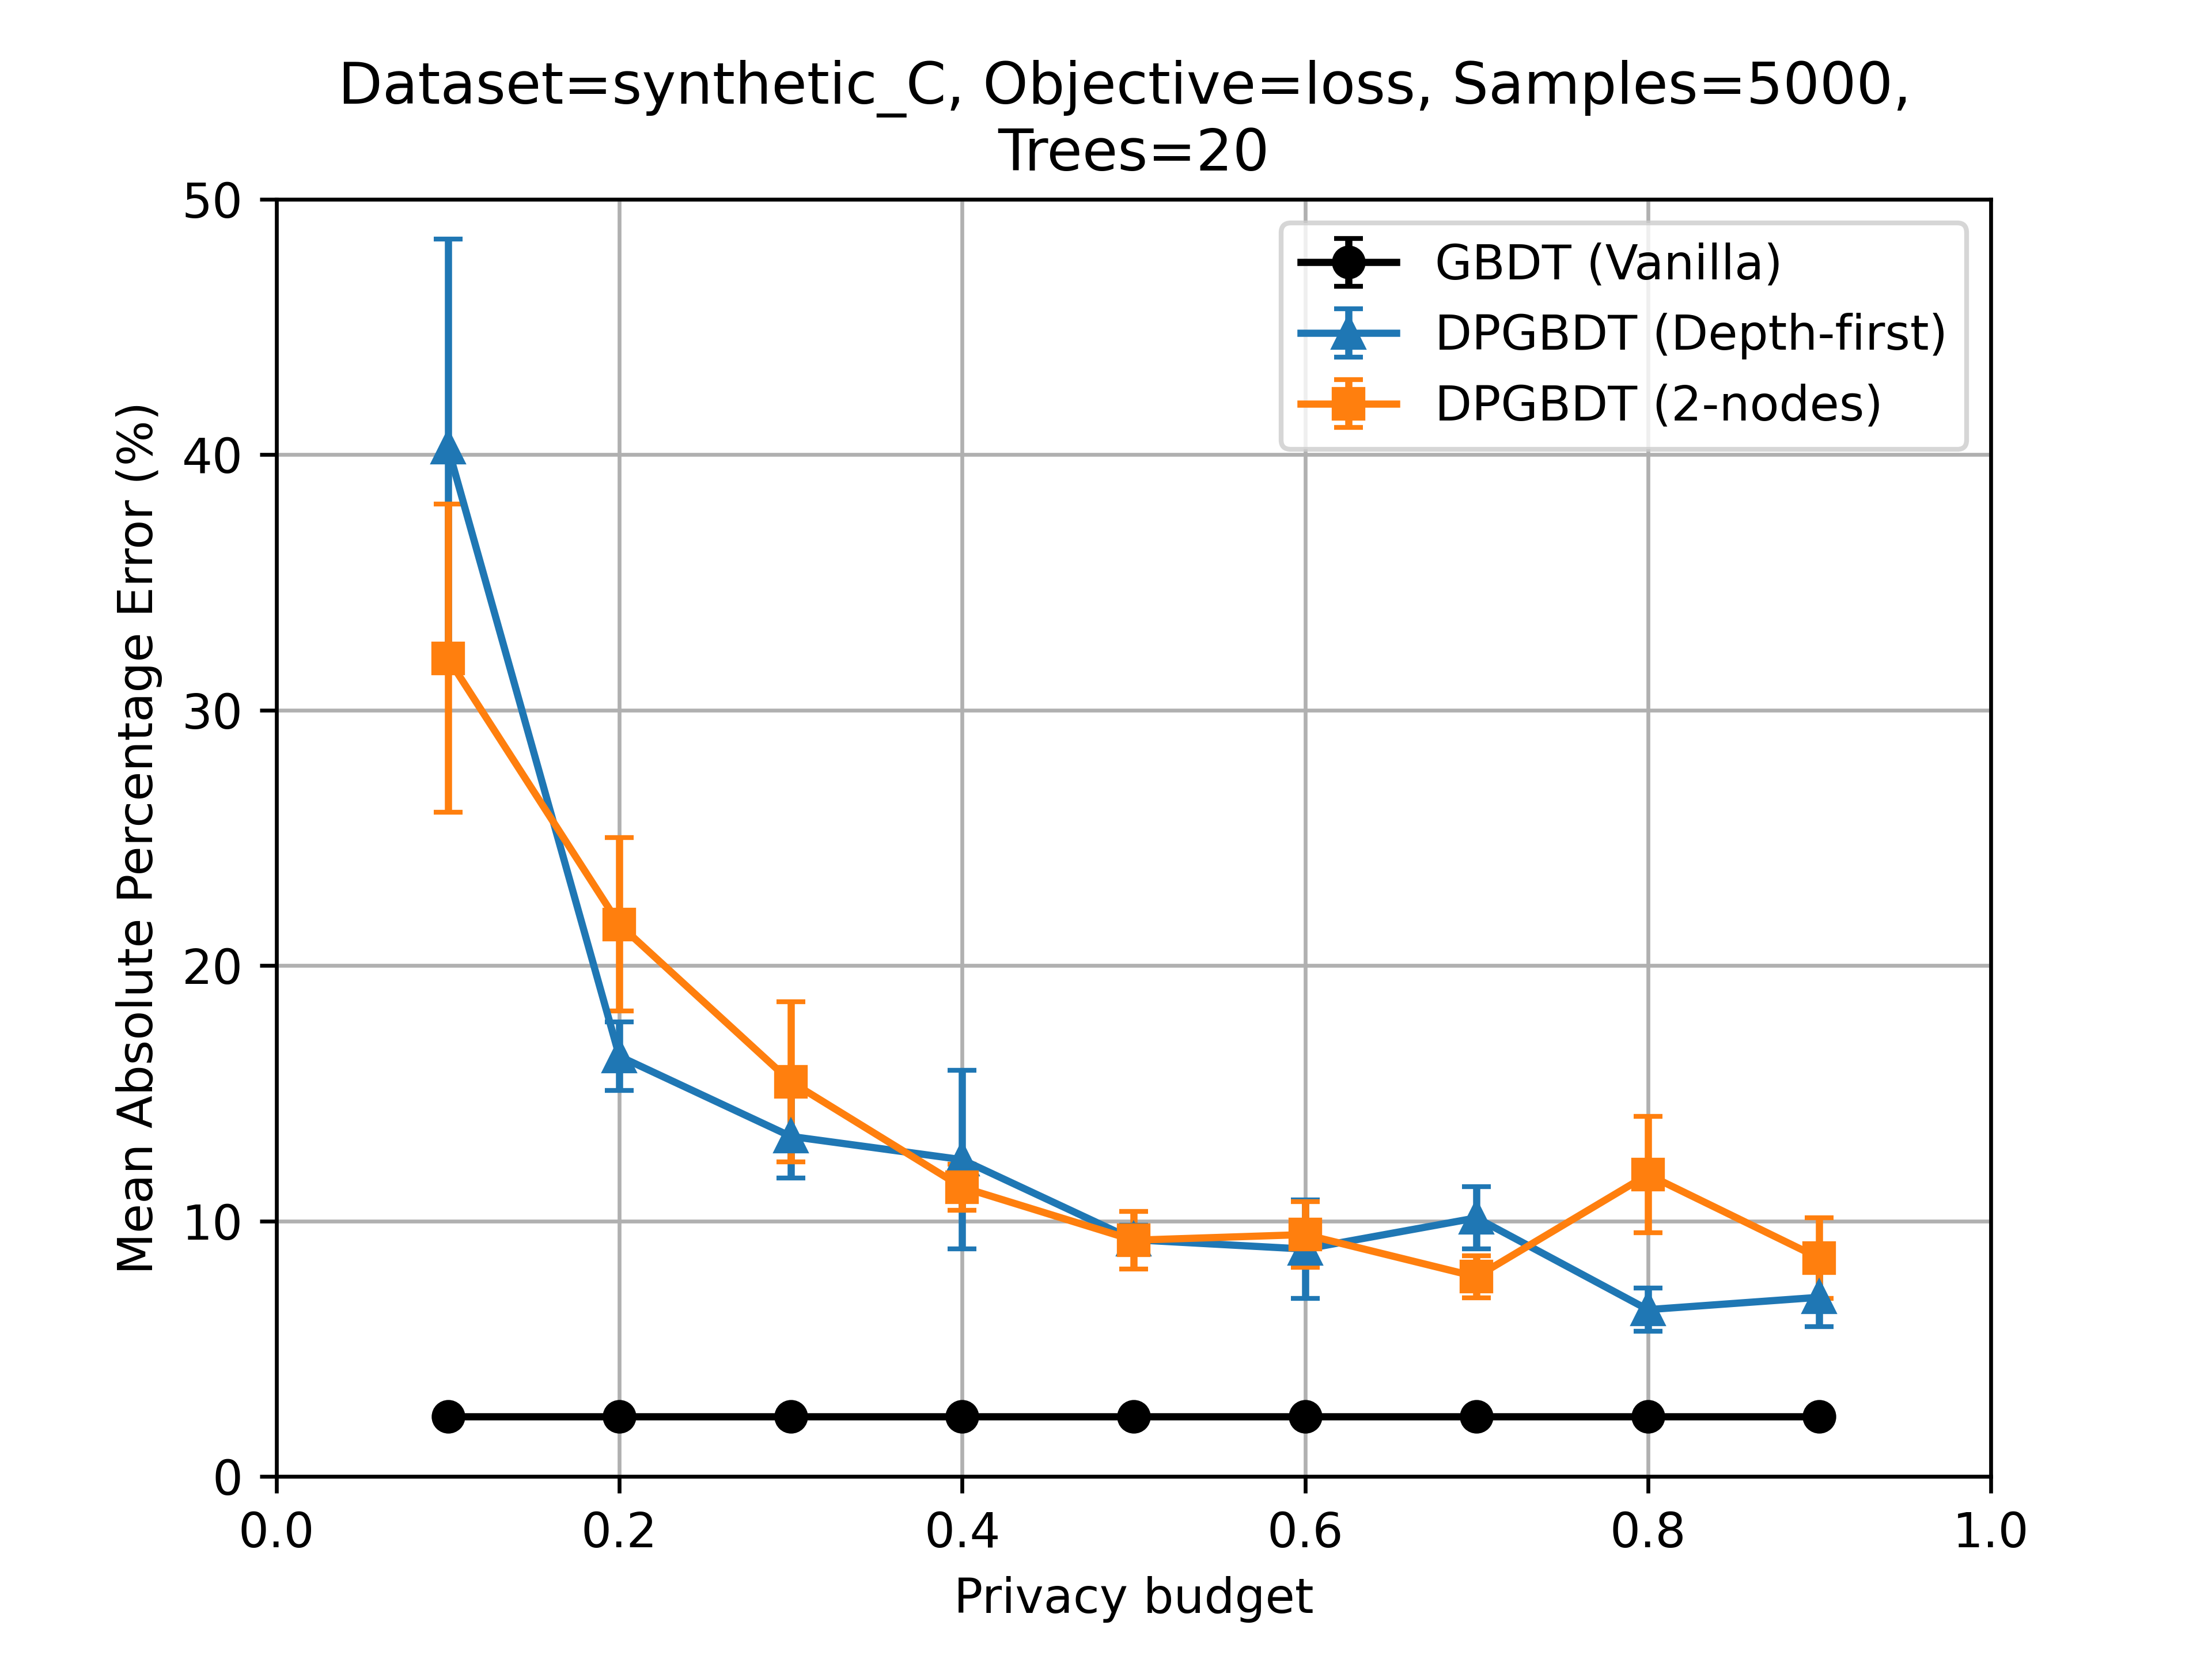
\includegraphics[width=.5\linewidth]{images/evaluation/synthetic_C_loss_5000.png}\hfill
  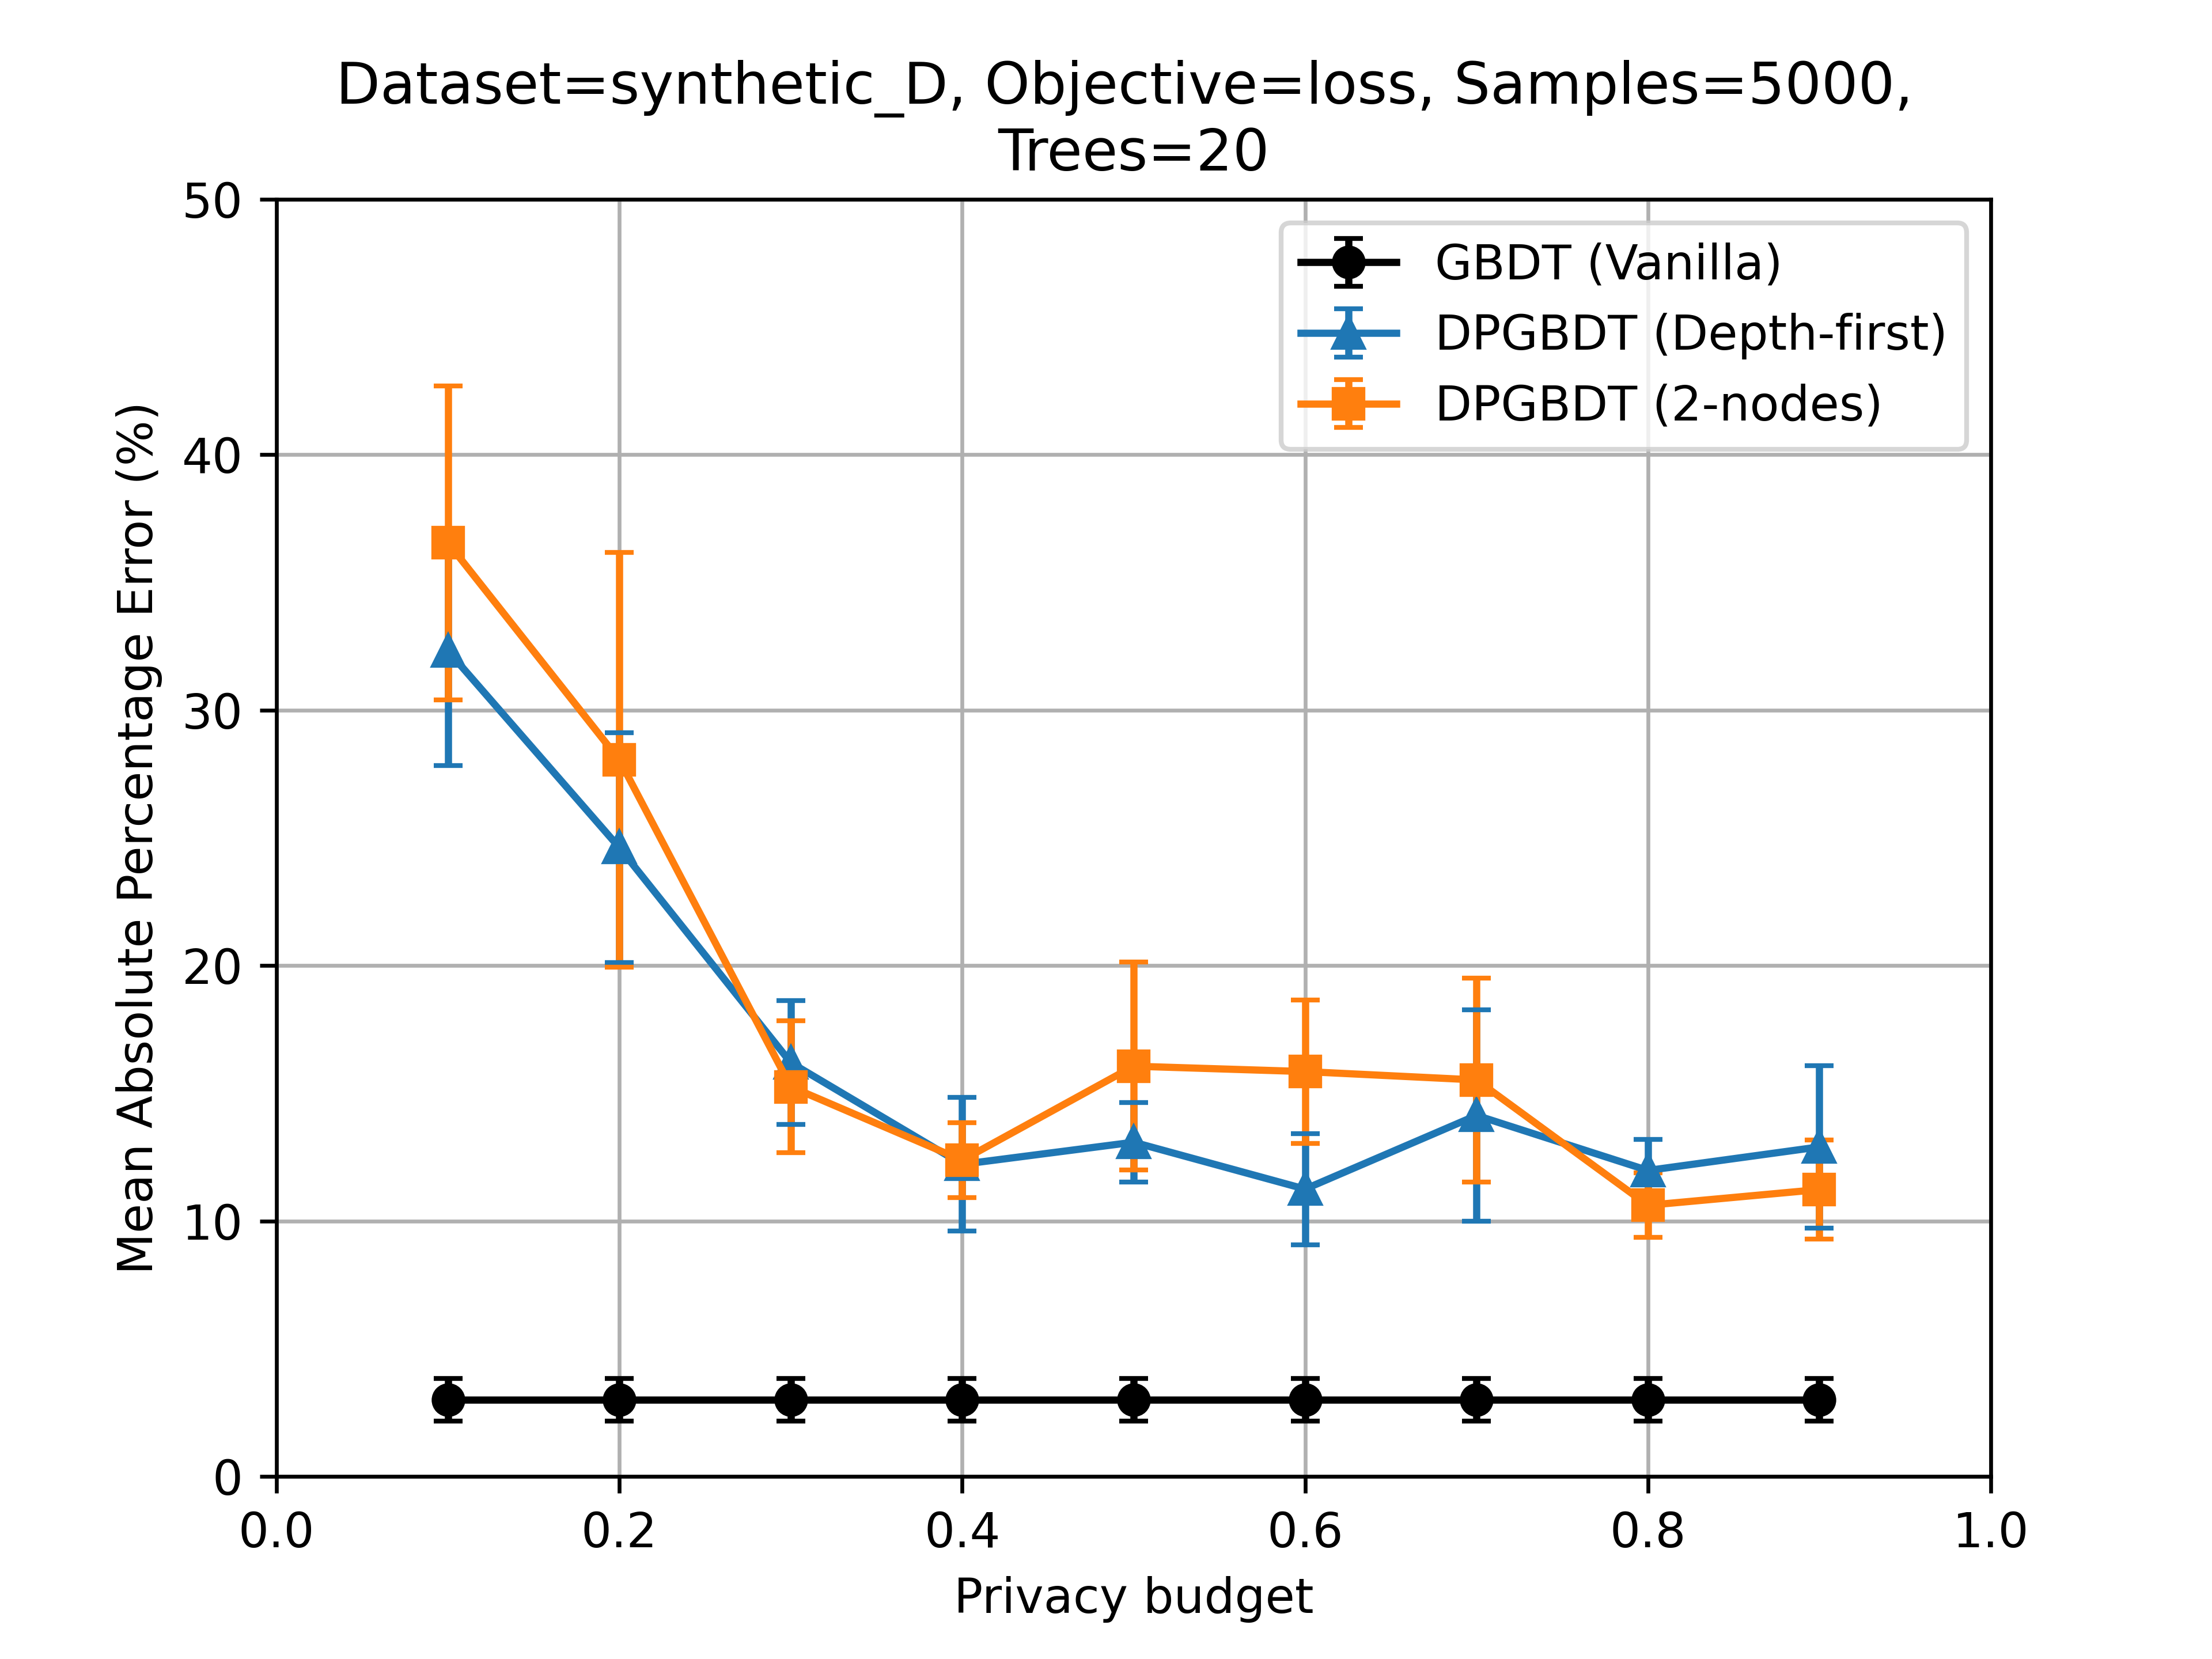
\includegraphics[width=.5\linewidth]{images/evaluation/synthetic_D_loss_5000.png}
  \caption{Synthetic datasets C and D}
  \end{subfigure}
  \caption{\label{fig:results_synthetic_loss}Mean Absolute Percentage Error for the \textit{loss} target on the synthetic datasets.}
\end{figure}

\begin{center}\begin{table}[h!]
	\center
	\noindent\makebox[0pt]{}{
		\begin{tabular}{|c|c|c|c|}
 		\hline
 		 & (Non-DP) Vanilla & (DP) Depth-first & (DP) 2-nodes \\ [0.5ex] \hline\hline
 		Synthetic A & $74.06$ & $\textbf{41.87}$  & $44.89$ \\ \hline
 		Synthetic B & $74.02$ & $47.77$  & $\textbf{47.31}$ \\ \hline
 		Synthetic C & $73.48$ & $\textbf{45.36}$  & $51.08$ \\ \hline
 		Synthetic D & $73.70$ & $51.16$  & $\textbf{47.89}$ \\ \hline
	\end{tabular}
	\caption{\label{table:attack_cost}Membership inference attack success rate (in $\%$) for the \textit{cost} target on the synthetic datasets. Train-test split is set to 75-25\%.}}
\end{table}\end{center}

\begin{figure}[h!]
  \begin{subfigure}{\linewidth}
  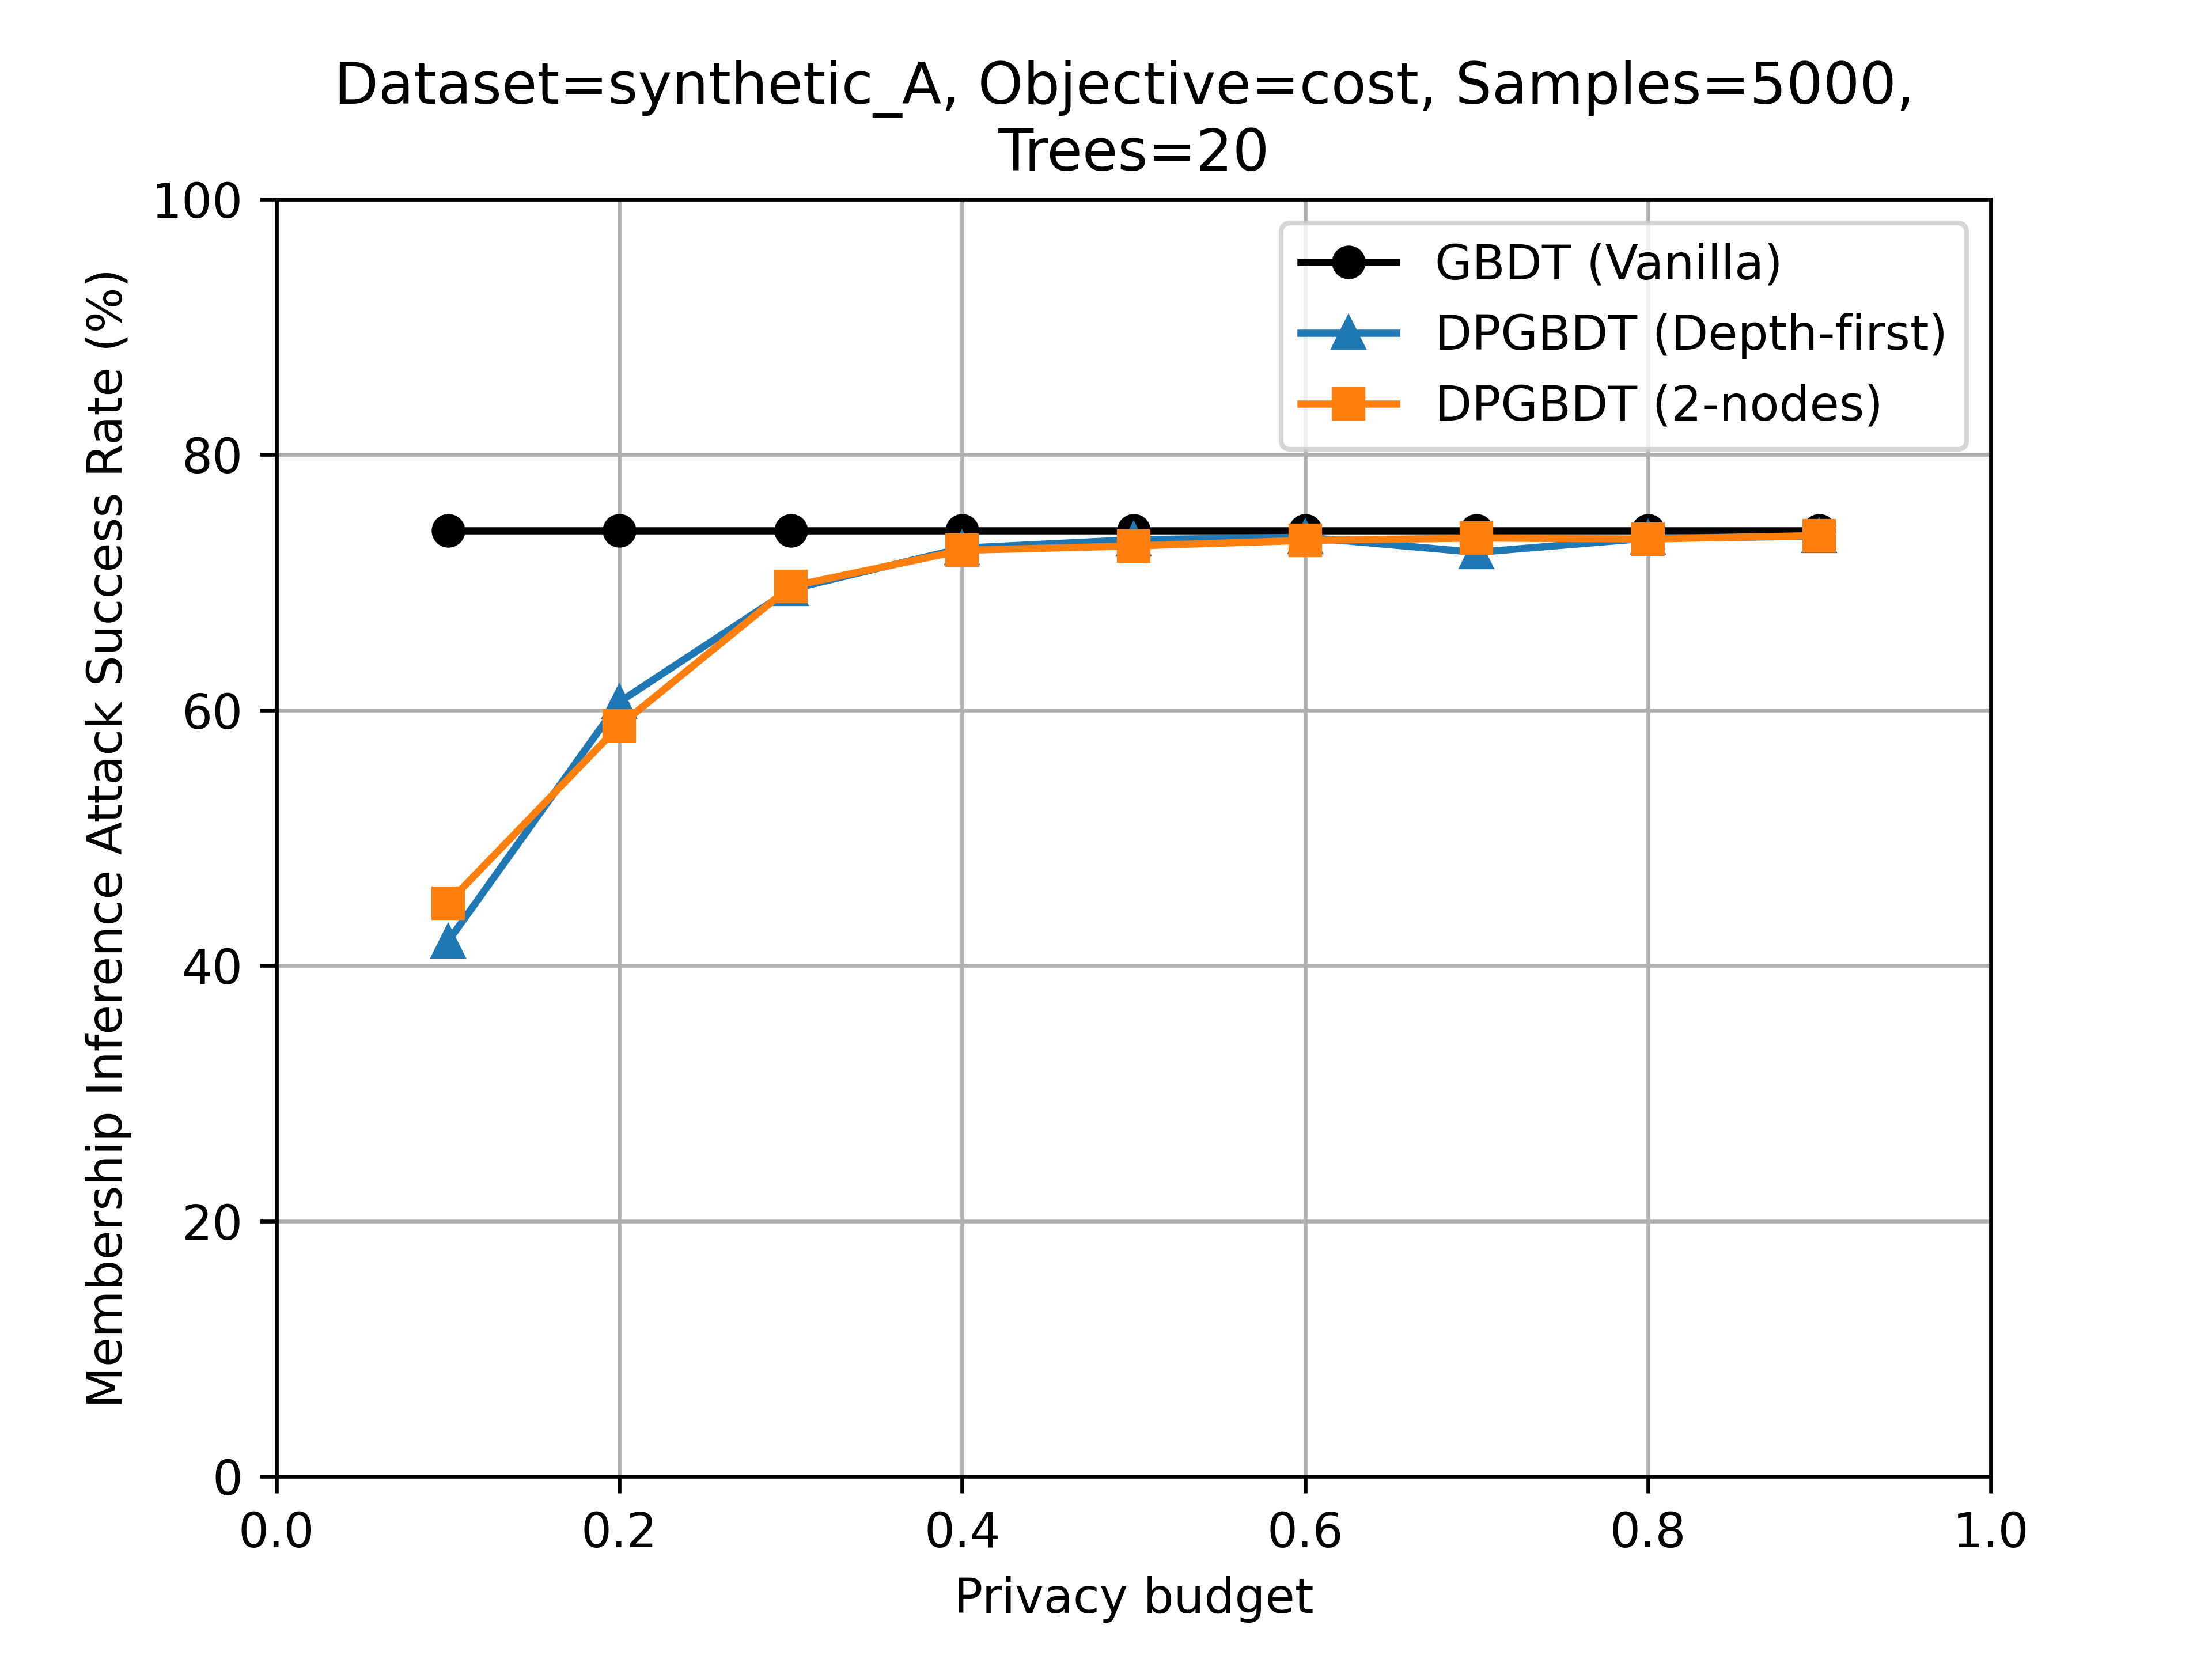
\includegraphics[width=.5\linewidth]{images/evaluation/attack_synthetic_A_cost_5000.png}\hfill
  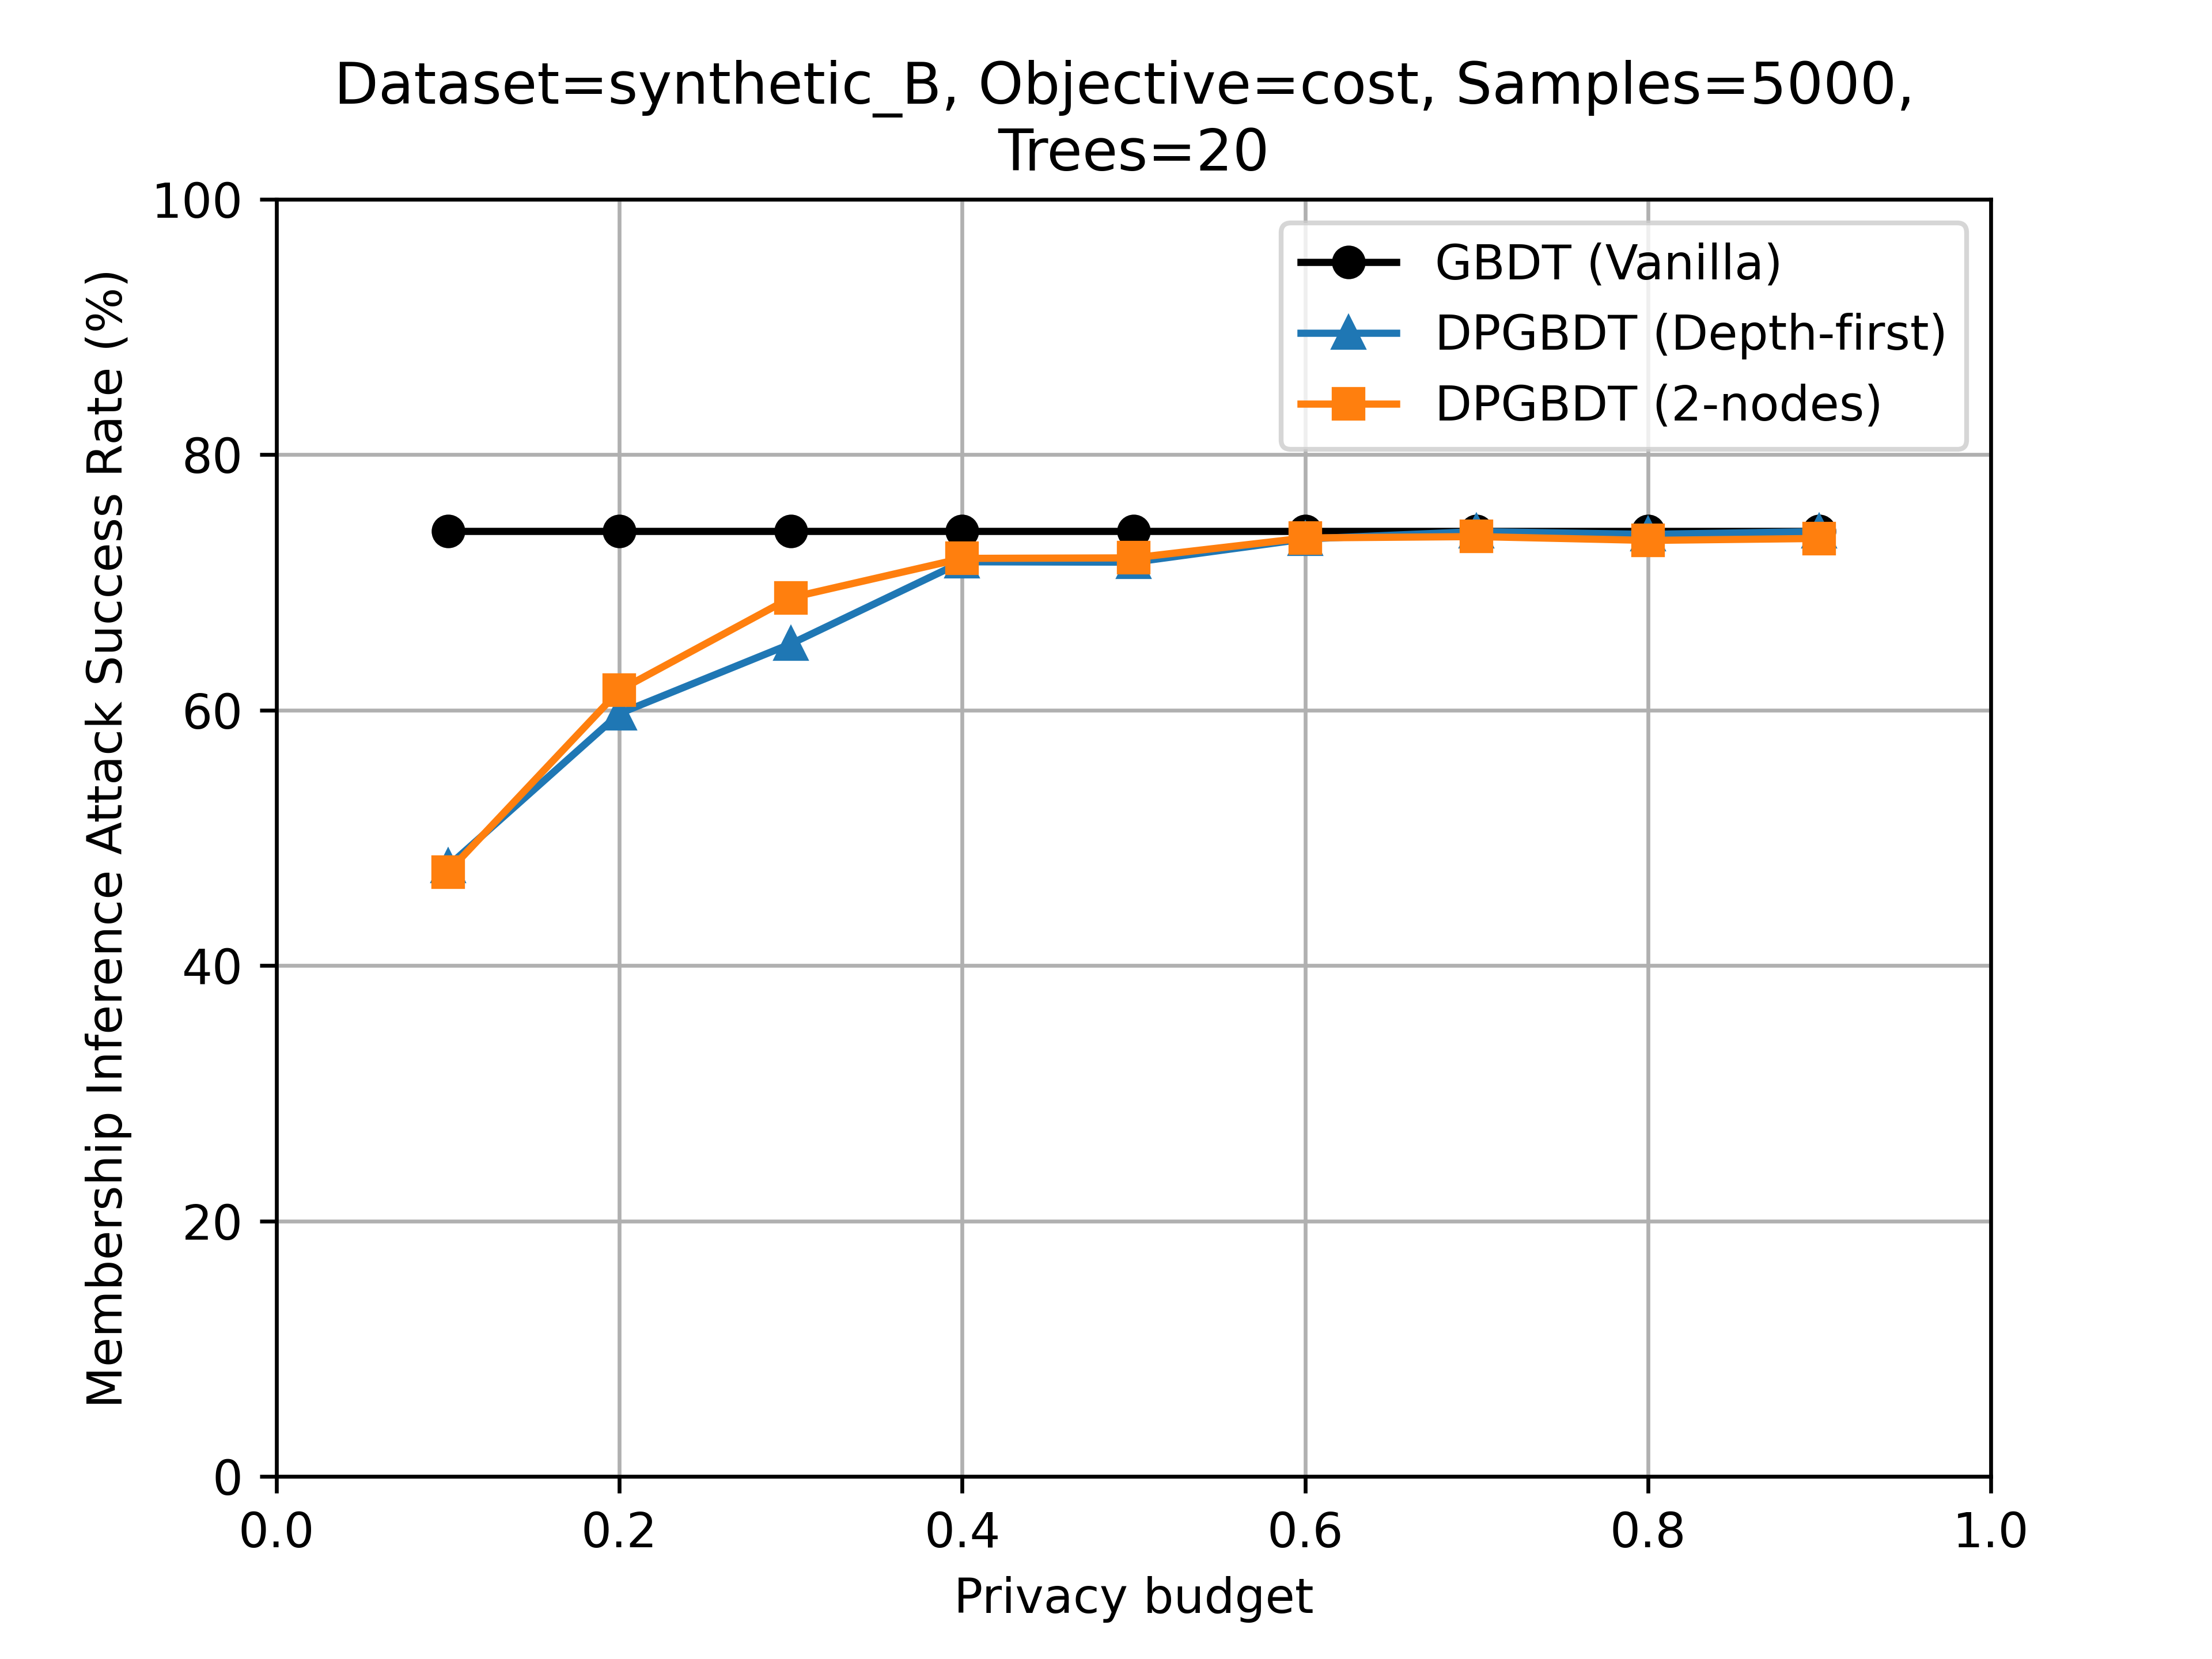
\includegraphics[width=.5\linewidth]{images/evaluation/attack_synthetic_B_cost_5000.png}
  \caption{Synthetic datasets A and B}
  \end{subfigure}\par\medskip
  \begin{subfigure}{\linewidth}
  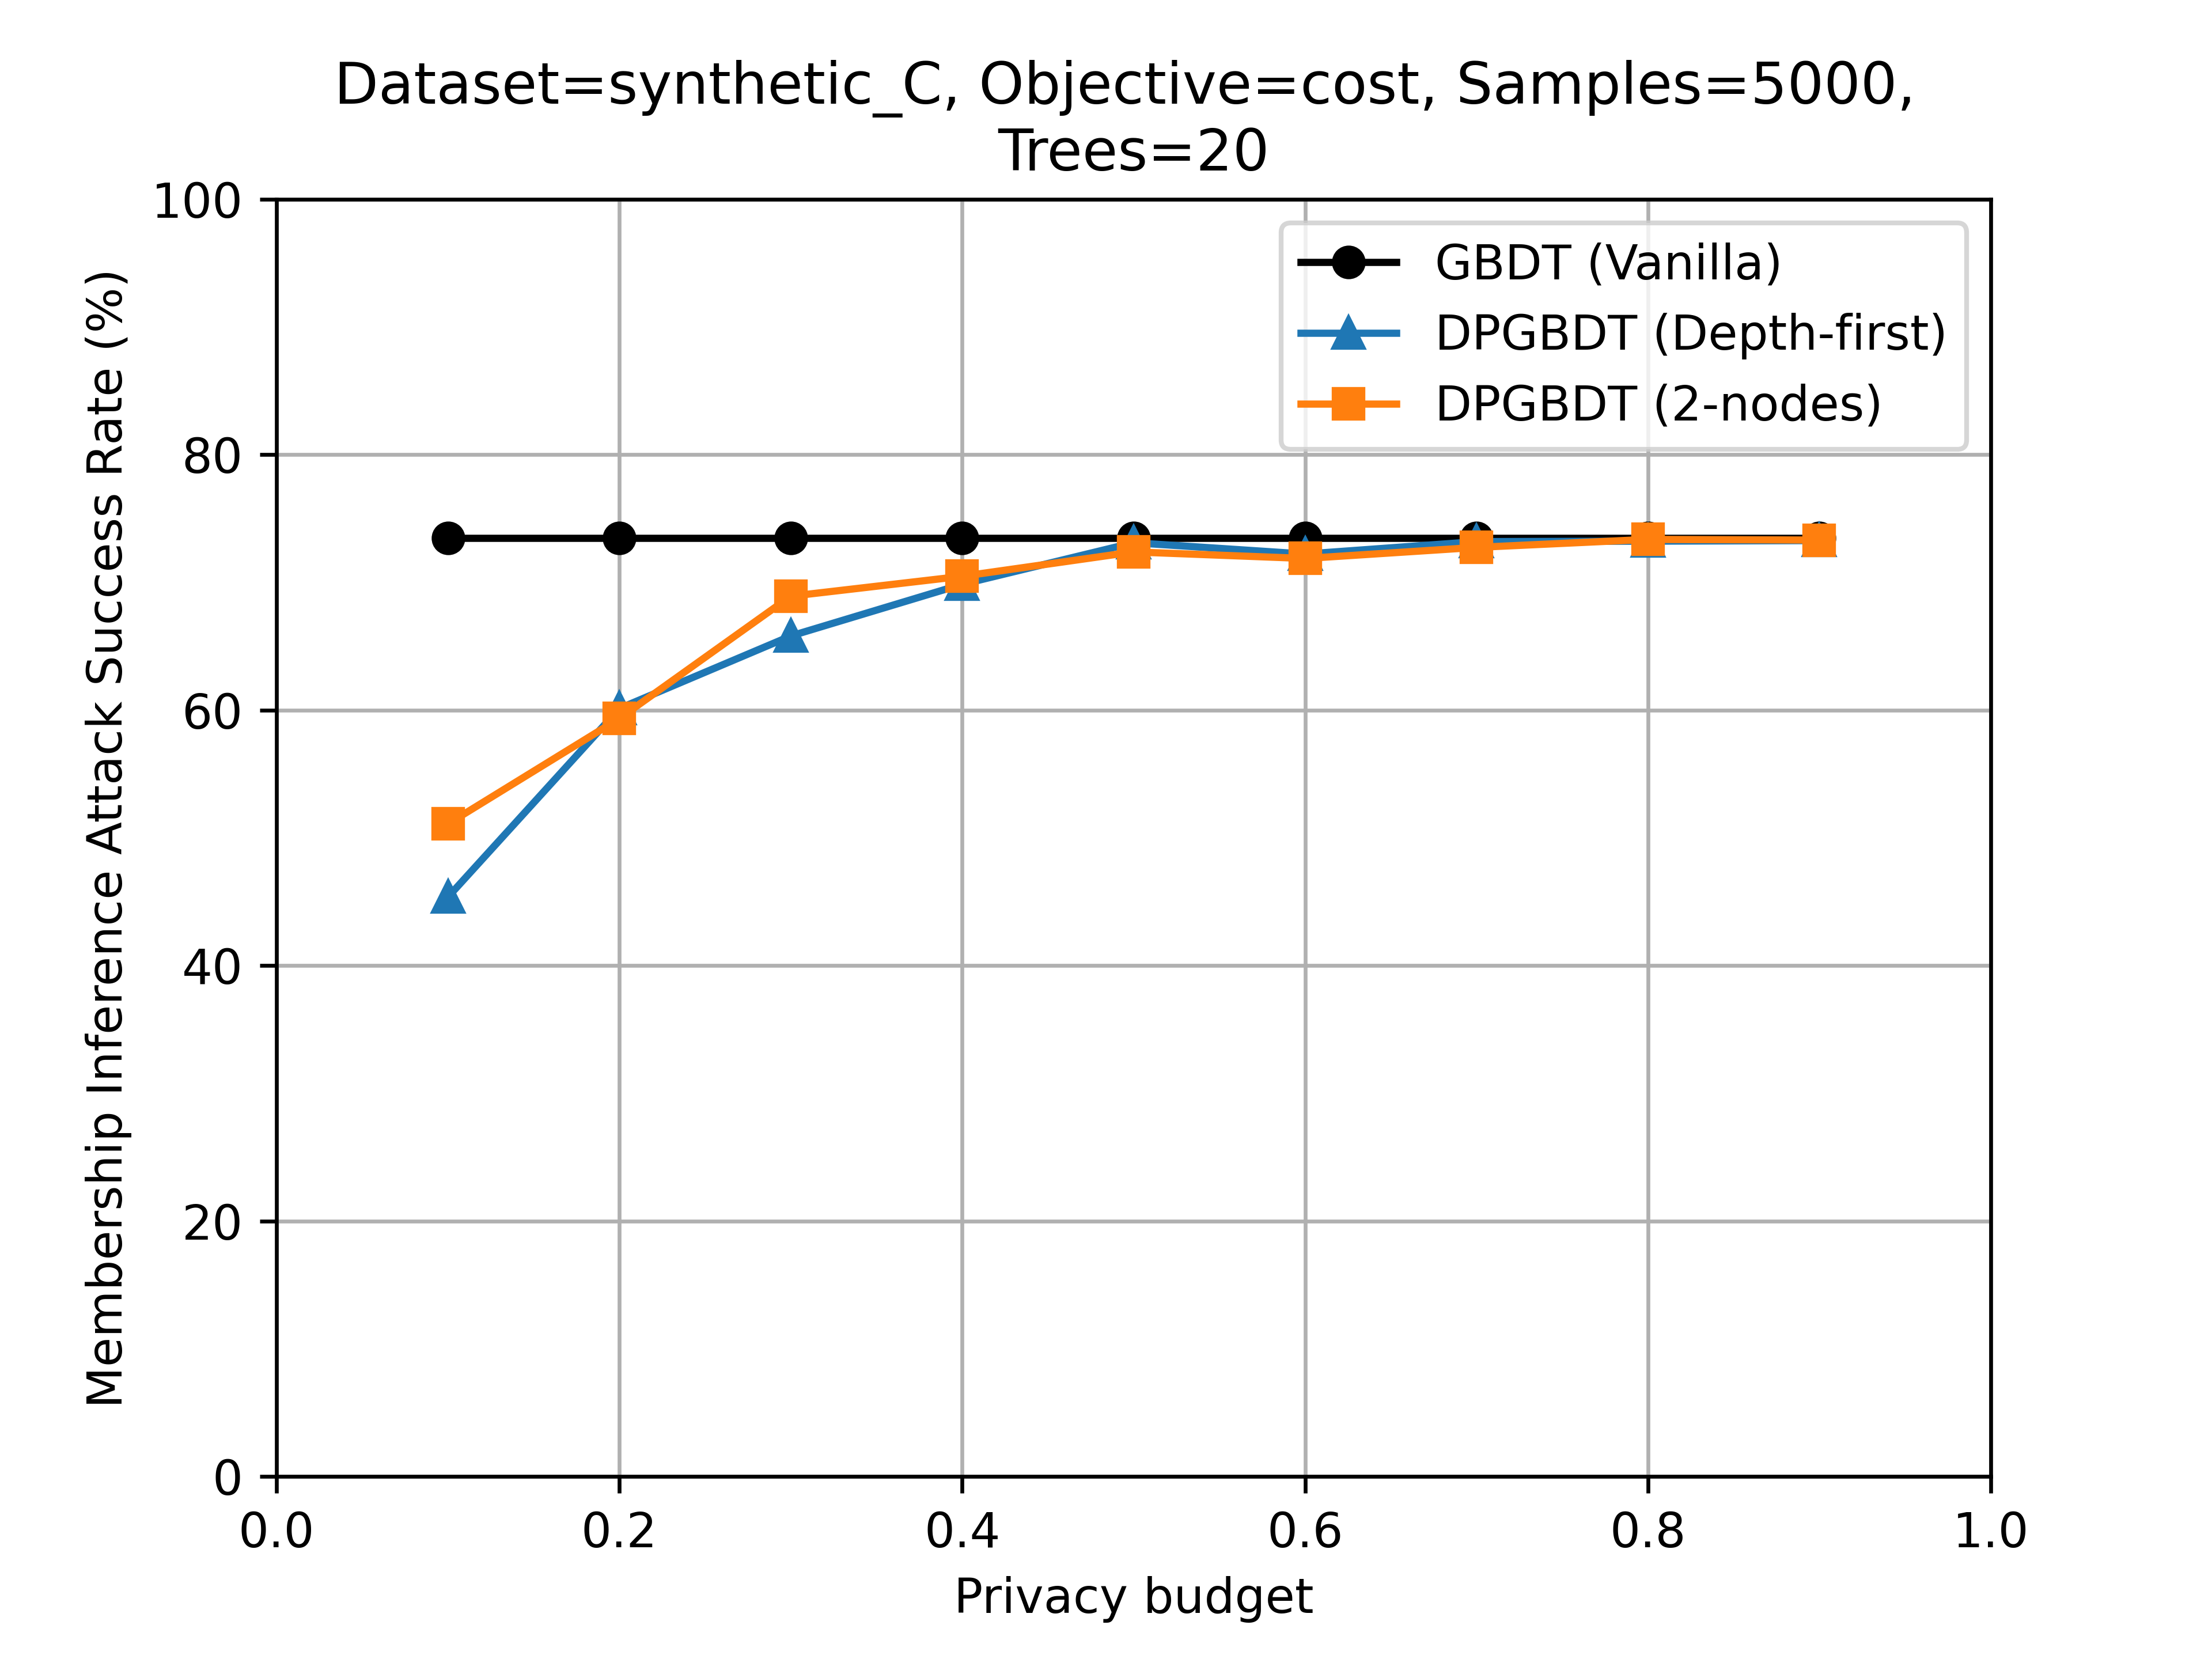
\includegraphics[width=.5\linewidth]{images/evaluation/attack_synthetic_C_cost_5000.png}\hfill
  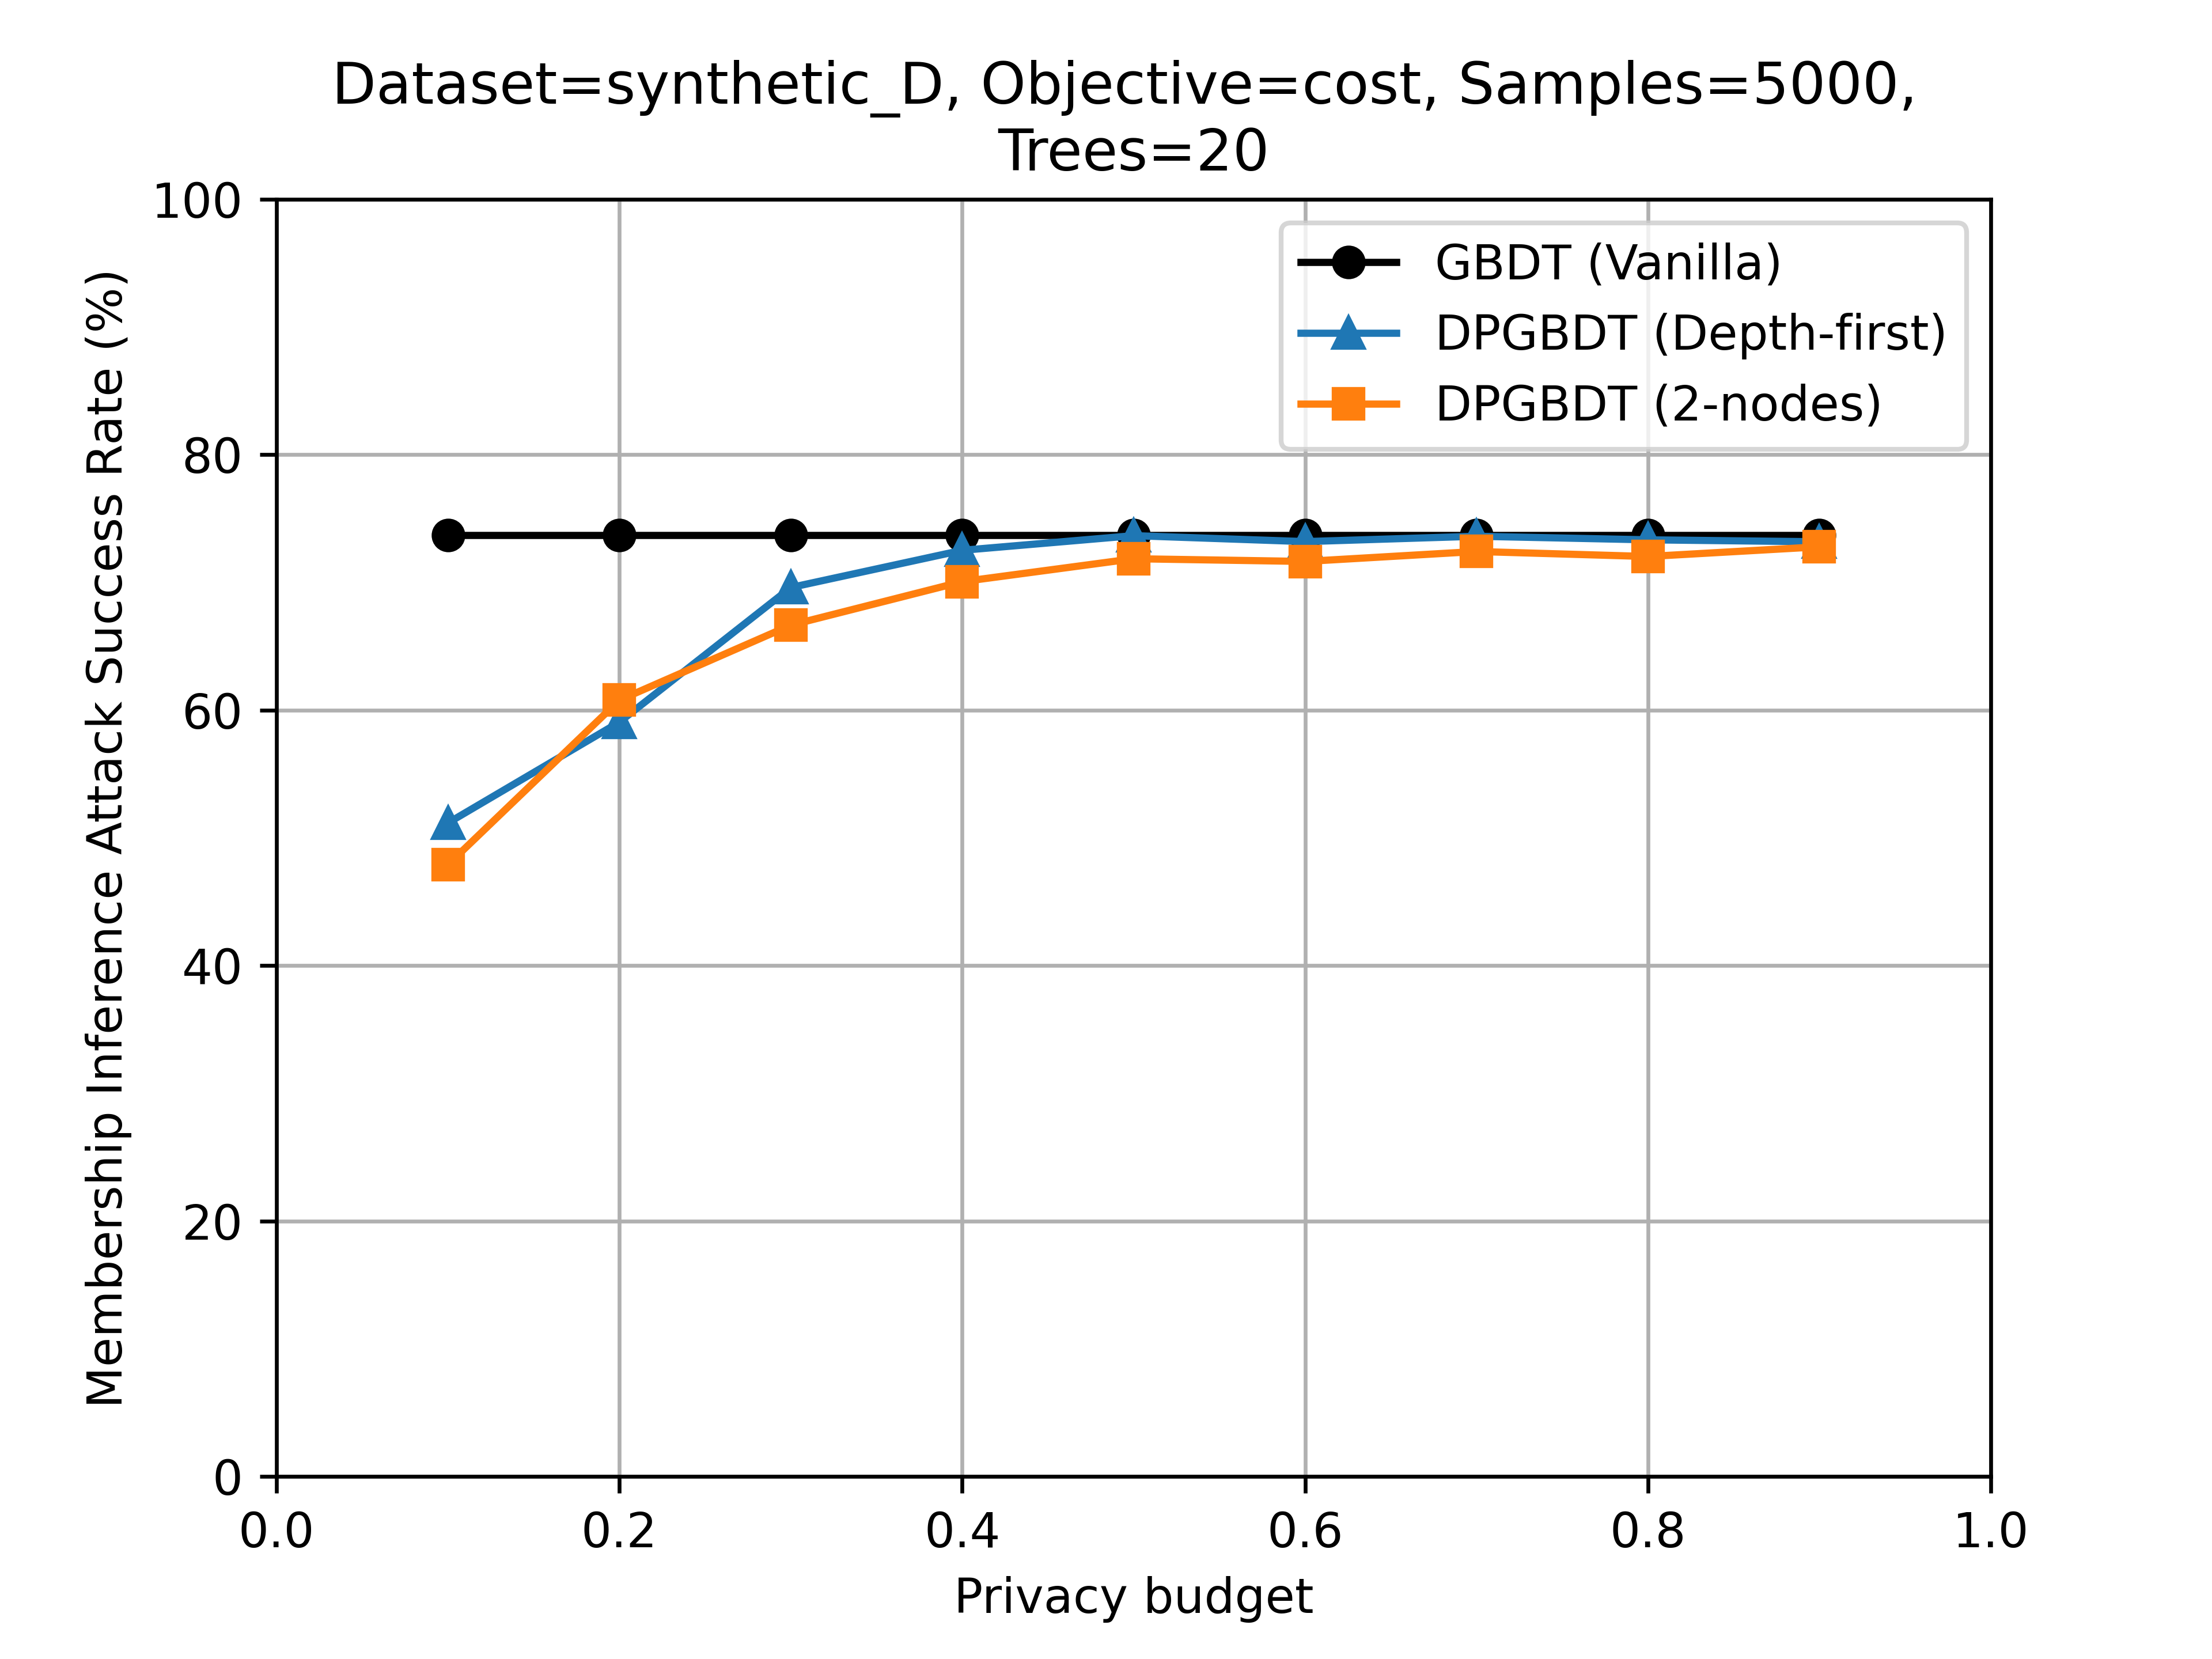
\includegraphics[width=.5\linewidth]{images/evaluation/attack_synthetic_D_cost_5000.png}
  \caption{Synthetic datasets C and D}
  \end{subfigure}
  \caption{\label{fig:attack_cost}Membership inference attack success rate (in $\%$) for the \textit{cost} target on the synthetic datasets. Train-test split is set to 75-25\%.}
\end{figure}

\begin{figure}[h!]
  \begin{subfigure}{\linewidth}
  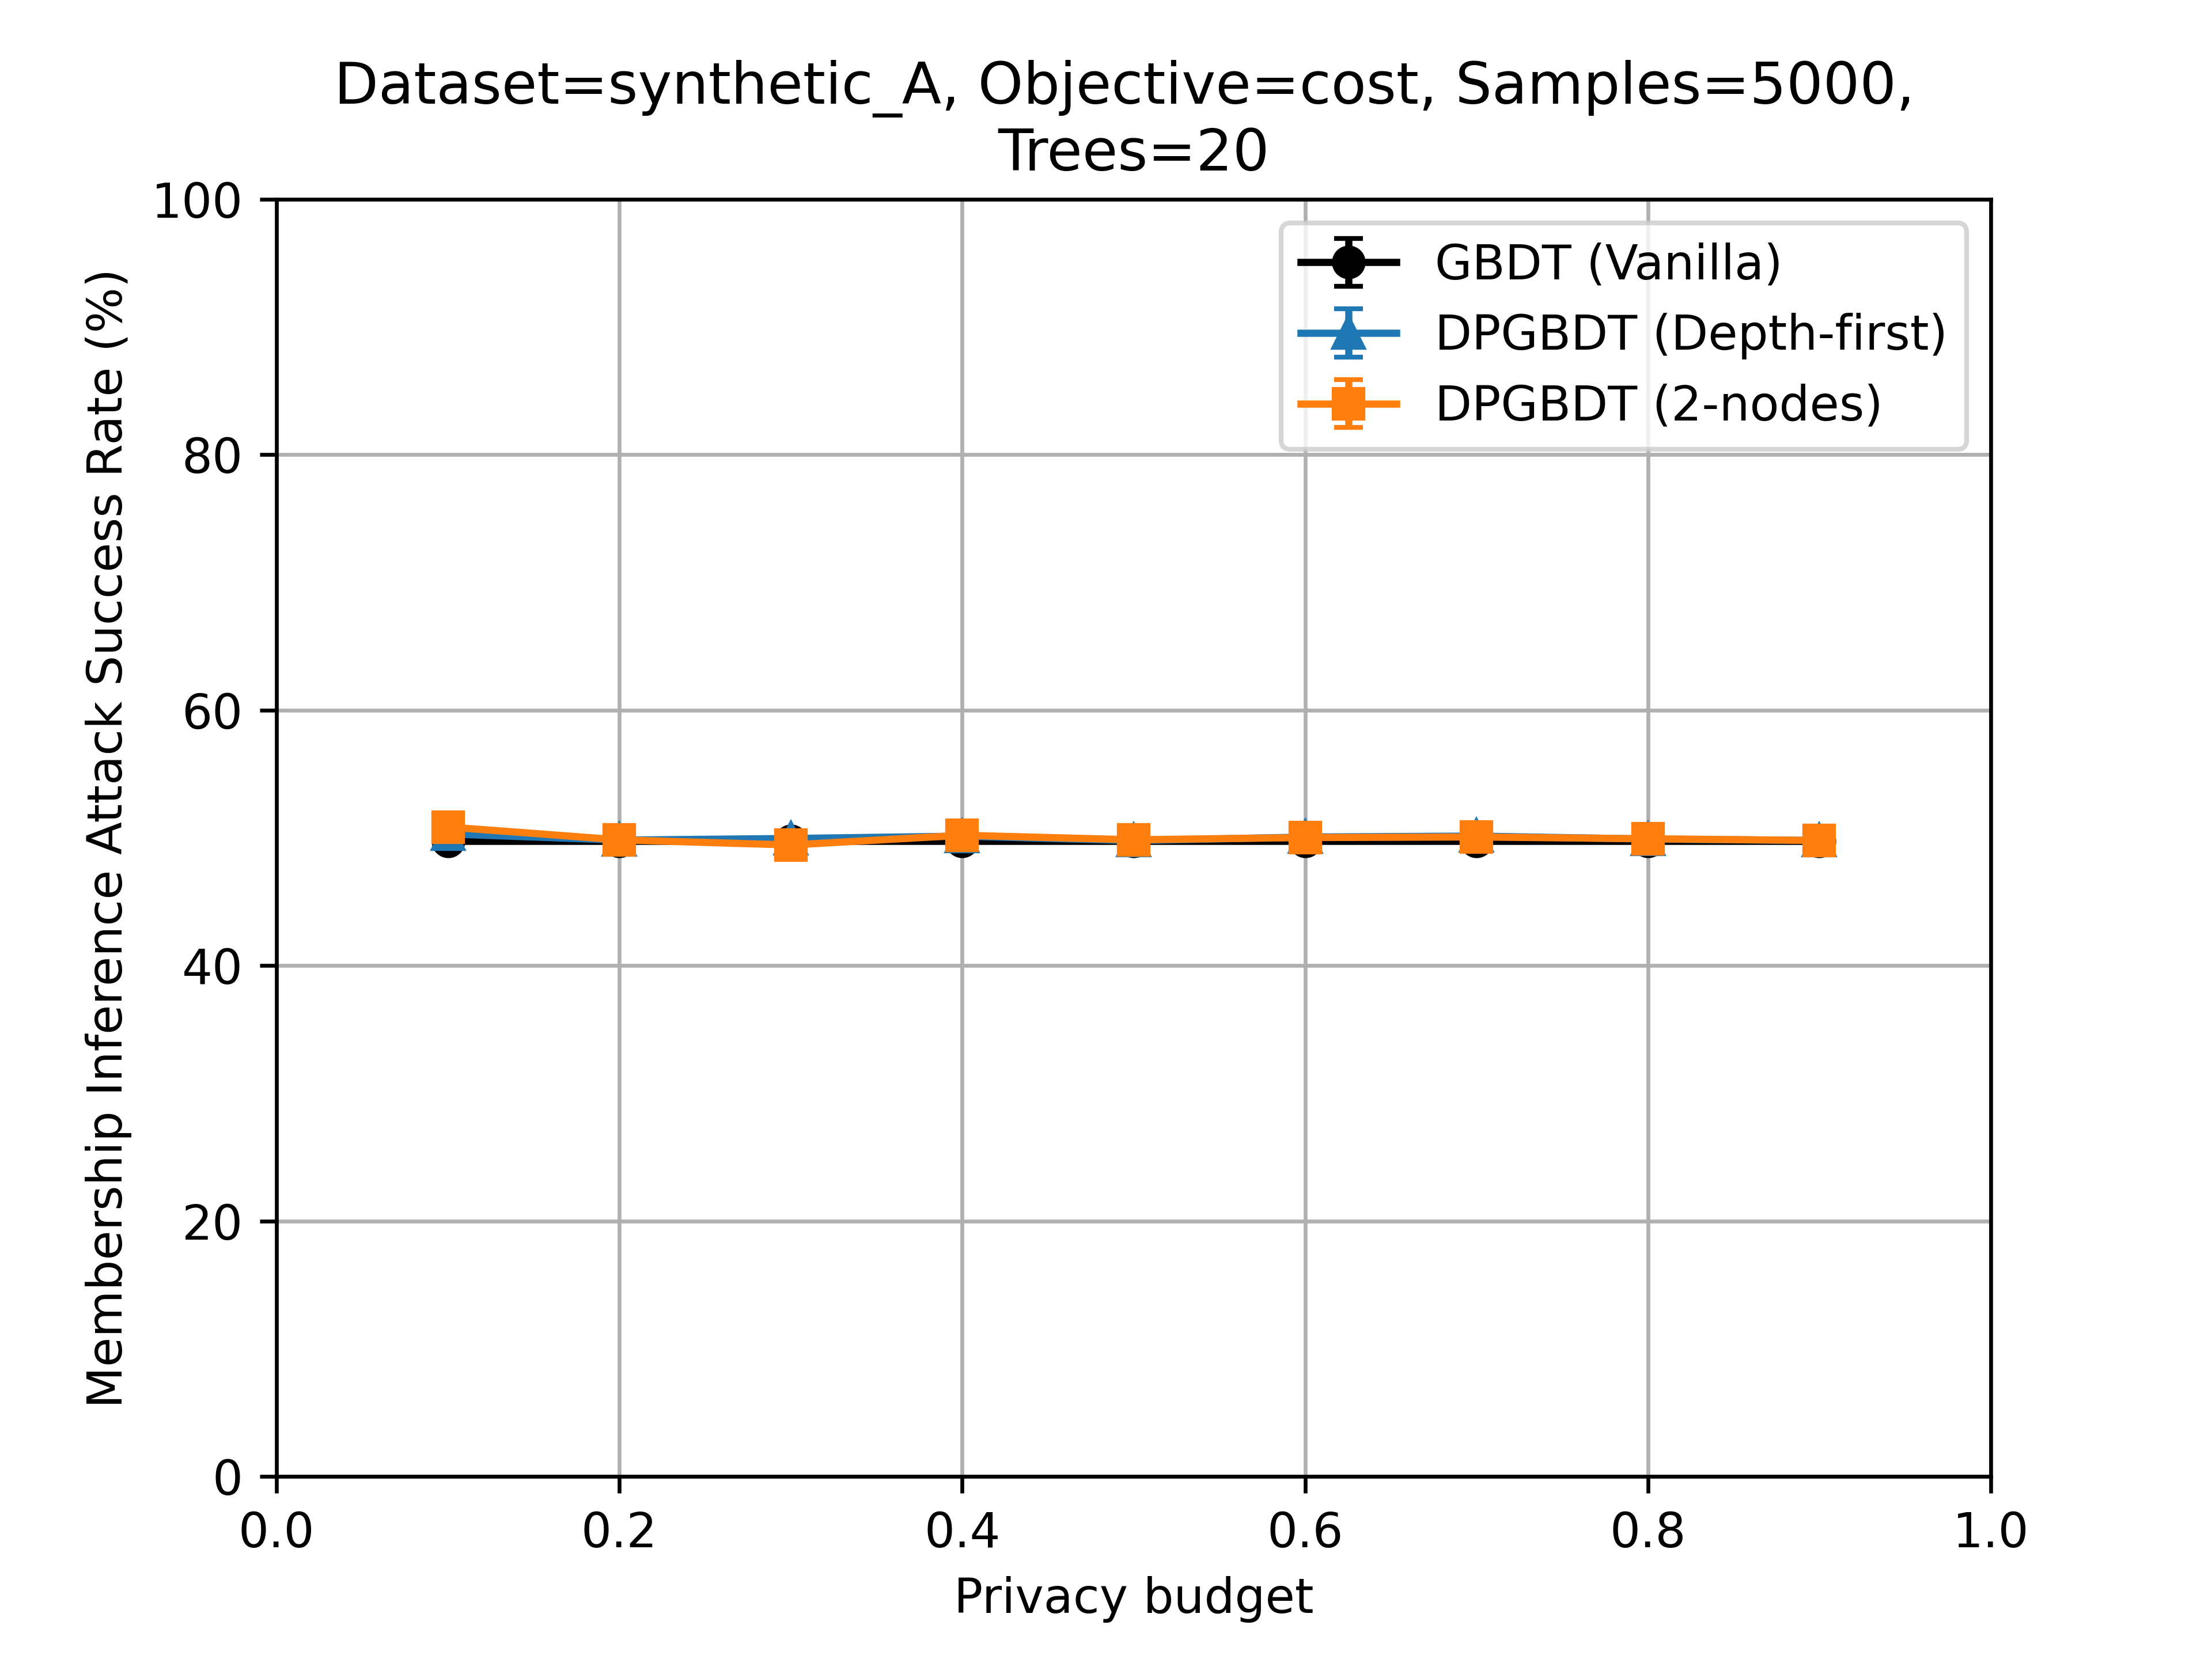
\includegraphics[width=.5\linewidth]{images/evaluation/5050-attack_synthetic_A_cost_5000.png}\hfill
  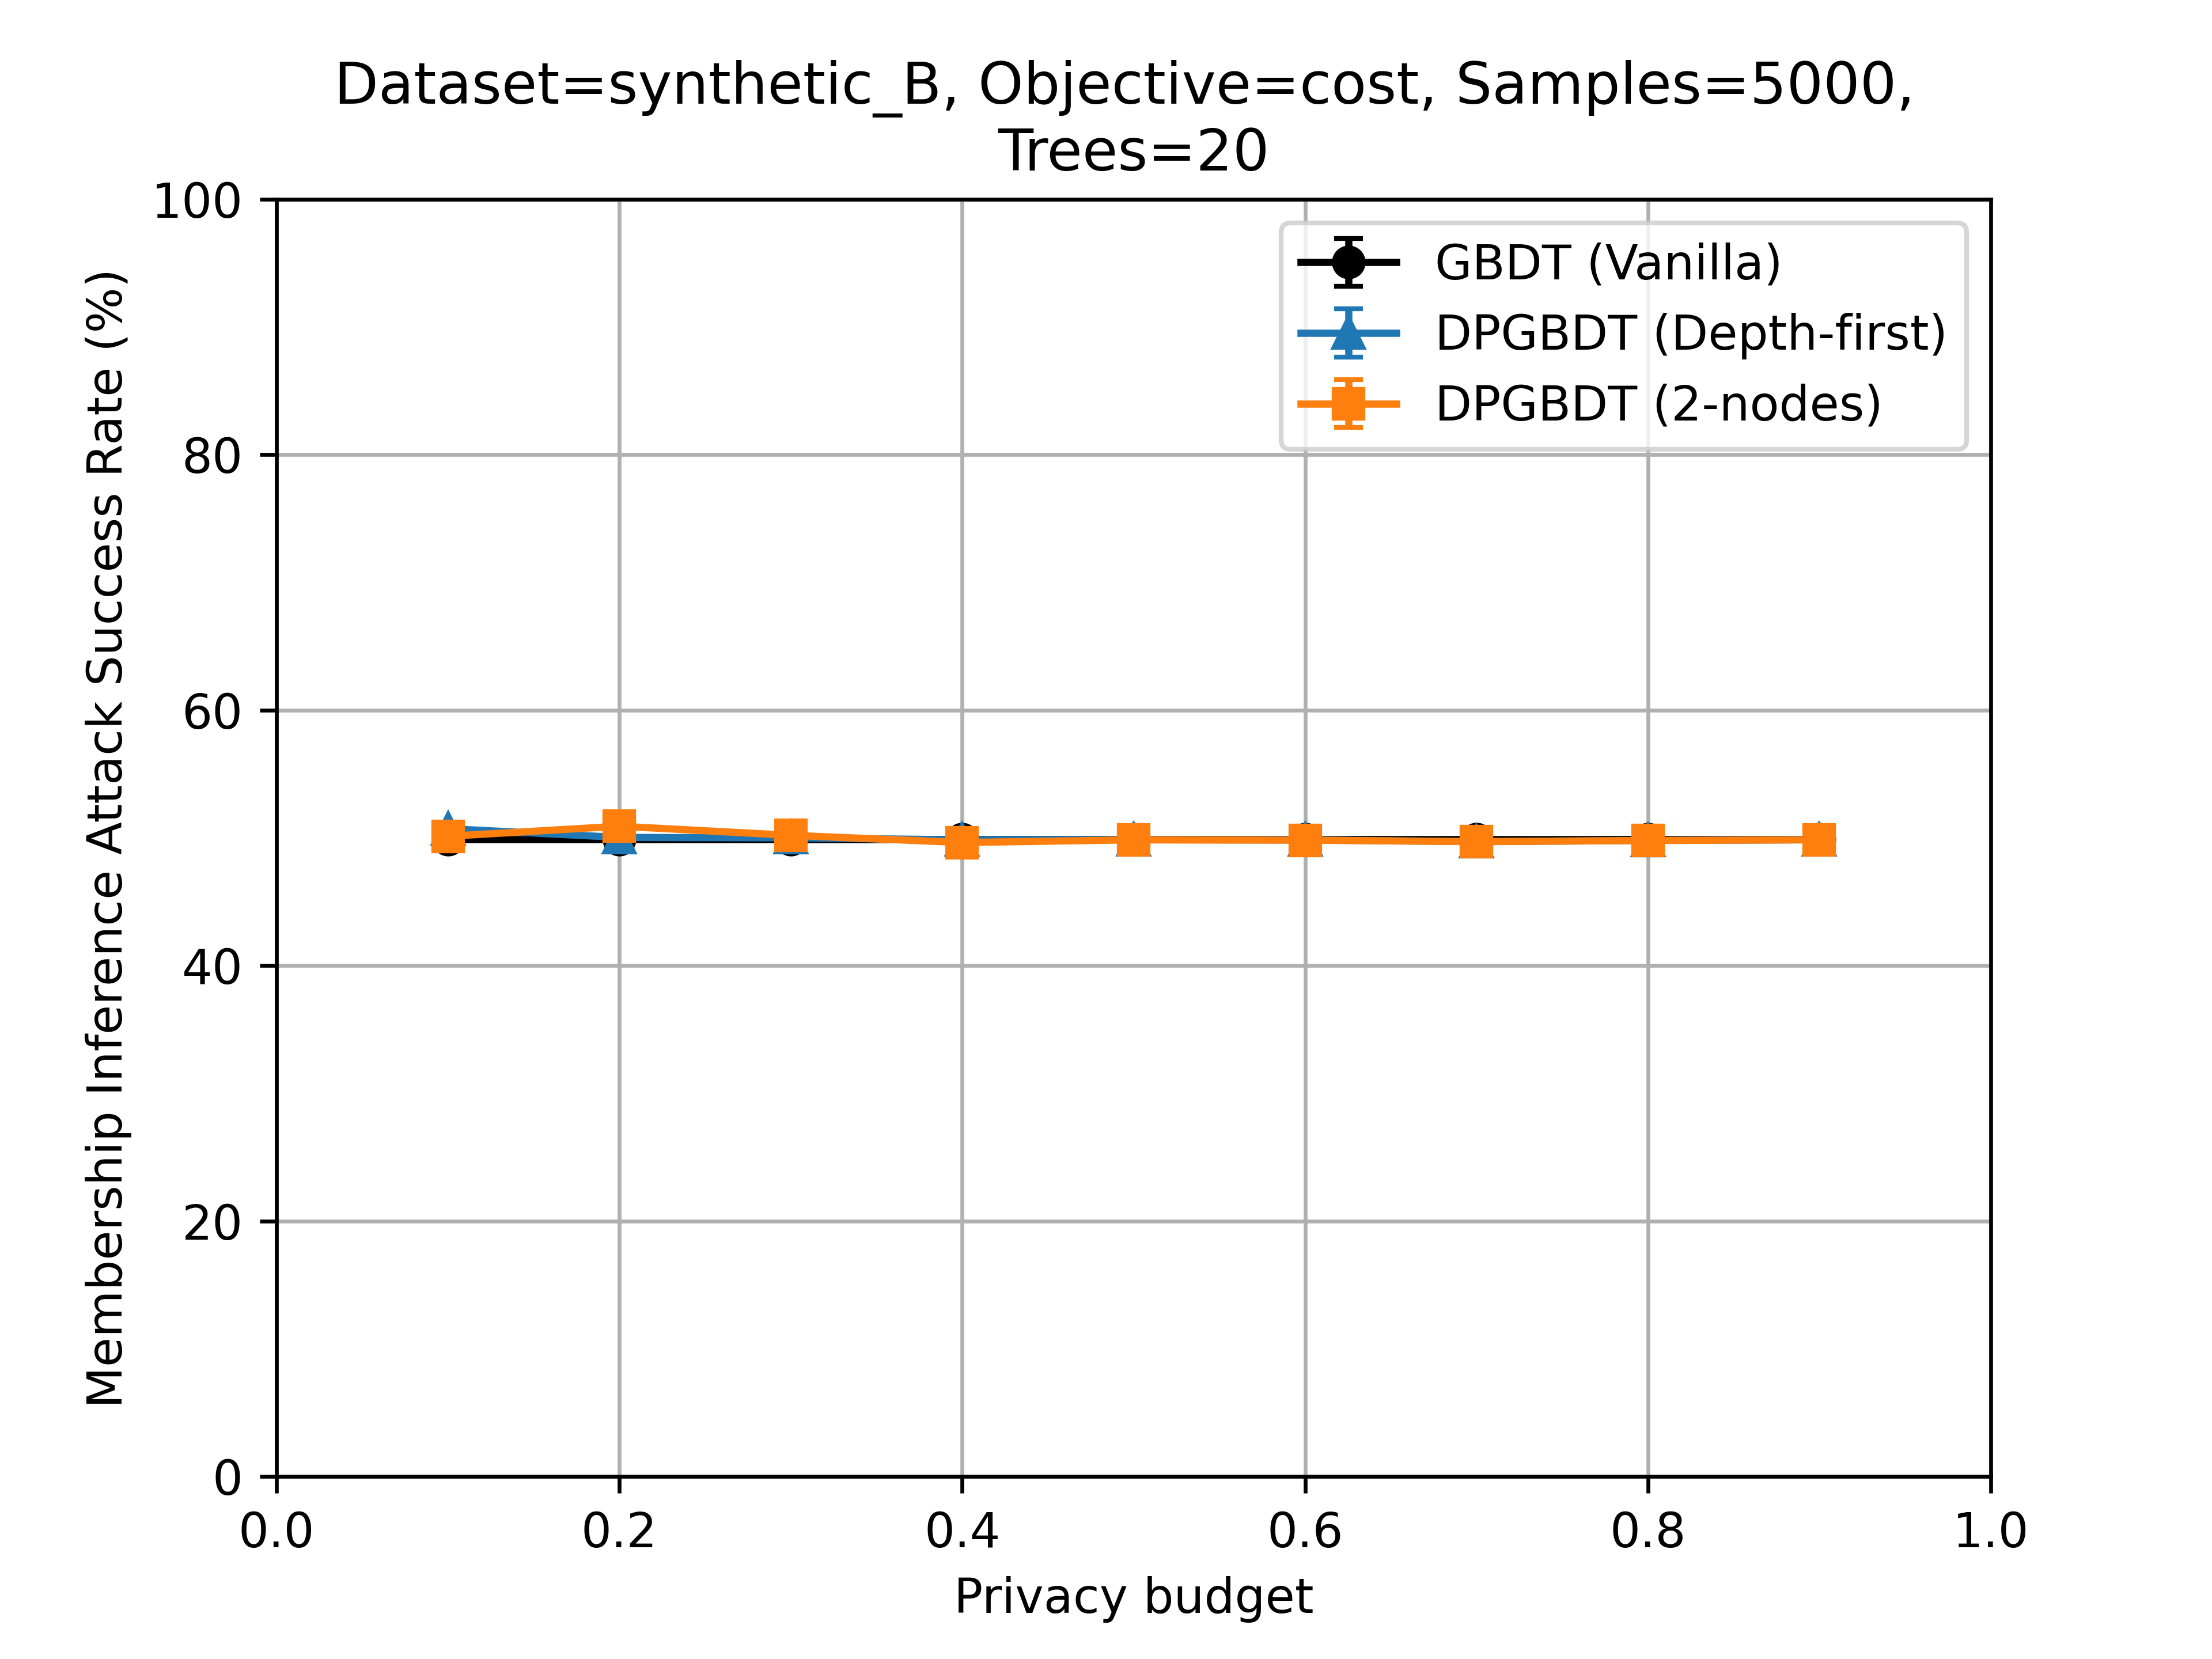
\includegraphics[width=.5\linewidth]{images/evaluation/5050-attack_synthetic_B_cost_5000.png}
  \caption{Synthetic datasets A and B}
  \end{subfigure}\par\medskip
  \caption{\label{fig:attack_cost_50}Membership inference attack success rate (in $\%$) for the \textit{cost} target on the synthetic datasets. Train-test split is set to 50-50\%.}
\end{figure}
